\chapter{Background}\label{sec:background}

%============================= INTRODUCTION =================================
Machine learning is a complex subfield of AI that witnessed a very quick
expansion in the recent years. It aims to enable computers to \emph{learn} how
to tackle problems by detecting patterns and regularities in the training data
and trying to generalize this extracted knowledge to new, unseen data.
Among its many powerful tools, artificial neural networks are models that take
inspiration from what is known about the human brain, by mimicking its
connectivity patterns, learning rules and signal propagation, under the
constraints imposed by our limited knowledge of the brain and the intrinsically
different "hardware" at our disposal.

While it is beyond the scope of this document to give a formal and in-depth
introduction to every concept needed to fully comprehend machine learning,
the following sections will introduce Artificial Neural Networks (ANNs), with a
specific focus on two of the most used kinds of neural networks i.e.,
Convolutional Neural Networks (CNNs) and Recurrent Neural Networks (RNNs). The
interested reader can find a more detailed overview of machine learning and of
its subfield deep learning in the books by~\cite{bishop-book2006} and
\cite{Goodfellow-et-al-2016-Book} respectively.

%================================== SECTION ==================================
\section{Artificial neural networks}\label{sec:NN}
Biological brains are composed by a large number of simple elements, called
neurons, that are highly interconnected. The number of neurons in the human
brain is estimated to be around $10^{11}$, each one connected to a little less
than $10^{4}$ other neurons, resulting in a total between $10^{14}$ and
$10^{15}$ synapses~\citep{drachman2005we}. The activity of each of these either
excites or inhibits the surrounding neurons it is connected to, generating a
complex network of interactions. Artificial Neural Networks (ANNs) take
inspiration from this understanding of the human brain, building networks
composed of many artificial neurons, small elements that perform very simple
operations on their inputs.

\subsection{Brief history of neural networks}
In 1943 McCulloch and Pitts defined a mathematical model of how a biological
neuron works~\citep{McCulloch43}. The artificial neuron they proposed was
able to solve simple binary problems, but did not learn. In 1949~\cite{Hebb49}
suggested that humans learn by enhancing the neural pathways between neurons
that collaborate, and weakening the others. Only a decade later this learning
rule inspired the Perceptron~(see~\autoref{fig:perceptron}), the first ANN that
was able to vary its own weights, i.e., to find the setting that allowed it to
exhibit the desired behavior~\citep{Rosenblatt57}.

% PERCEPTRON
\begin{figure}[t]
    \centering
    \begin{neuralnetwork} [nodespacing=6mm, layerspacing=23mm,
            maintitleheight=2.5em, layertitleheight=5em,
            height=3, toprow=true, nodesize=17pt,
            style={}, title={}, titlestyle={}]

        %%%%% Layers
        \inputlayer[count=5, bias=true, title=Input\\layer, text=\nodetextxi]
        \outputlayer[count=1, text=\nodetextsigma]
        {\setdefaultlinklabel{\wilink}\linklayers}
        \redefinelayerspacing{18mm}
        \outputlayer[count=1, text=\nodetextstep]
        \linklayers
        \redefinelayerspacing{16mm}
        \outputlayer[count=1, text=\nodetexty]
        \linklayers
    \end{neuralnetwork}
    \centering
    \caption{\label{fig:perceptron}A representation of the Perceptron.}
\end{figure}

The activation rule of the perceptron is very simple and is at the base of many
modern neural networks. Given an $n$-dimensional input $\mathbf{x = (x_1,
\dots, x_n)}$, the weighted sum of each dimension of the input $x_i$ and its
associated weight $w_i$ is computed as

\begin{equation*}
    z = \sum_{i=1}^{n}(w_i \cdot x_i) + b,
\end{equation*}

\noindent where the weight $w_i$ is often referred to as \emph{preactivation}
and to simplify the notation the bias term $b$ will often be replaced by an
equivalent input term $x_0=1$ weighted by $w_0=b$. Note that this is simply the
dot product of the weight vector $\mathbf{w = (w_1, \dots, w_n)}$ and the input
vector $\mathbf{x}$. The result of this first affine transformation is then
passed through a step function of the form
\begin{equation*}
    y =
        \begin{cases}
            1,          & \text{if } z \geq 0 \\
            0,         & \text{otherwise},
        \end{cases}
\end{equation*}

% Although most modern ANNs apply a different nonlinear function
% (see~\autoref{sec:activation_fn}),
\noindent that determines the binary output of the Perceptron.

This can be used, for instance, to classify whether the input belongs to a
specific class or not. Note that the model can be easily extended to handle
multiple classes, by simply adding more dimensions to $y$ and assigning each of
them to a different class.

The behavior of the Perceptron is indeed remarkable, but the biggest innovation
of~\cite{Rosenblatt57} is most probably the update algorithm that allowed one
to modify the weights of the model. Given a training pair $(\mathbf{x}, y)$
consisting of an input and its corresponding desired output, the weights and
the bias -- also called the \emph{parameters} of the network -- are
\emph{learned} according to the following rule:

\begin{equation}\label{eq:perceptron_lr}
    w_i^{\text{new}} = w_i^{\text{old}} - \eta \cdot (\hat {y} - y) \cdot x_i,
\end{equation}

\noindent where $\hat y$ is the output of the Perceptron, $y$ is the target
(i.e., desired) value, $x_i$ and $w_i^{\text{old}}$ are respectively the $i$-th
input and weight at the previous iteration and $\eta$ is a scaling factor that
allows to adjust the magnitude by which the weights are modified.

The introduction of a model that could learn from data
%This discovery
was welcomed with excitement as the beginning of a new era and
research in ANNs became very active for approximately a decade, until in
1969 Minsky and Papert published a detailed mathematical analysis of the
Perceptron, demonstrating that a single layered Perceptron could not model
basic operations like the XOR logic operation~\citep{Minsky69}. The limit of
Perceptrons is that they can only solve linearly separable problems, and fail
at tackling nonlinearly separable problems like the
XOR~(see~\autoref{fig:XOR}). This is not the case for Multi-Layer
Perceptrons~(MLP, depicted in~\autoref{fig:MLP}), an evolution of Perceptrons
that introduces one or more intermediate layers (called \emph{hidden layers})
between the input and the output. Since Since in each of these layers the
preactivation is followed by a nonlinearity, the result is a nonlinear
transformation that can project the input into a linearly separable space.

\begin{figure}[t]
    \centering
    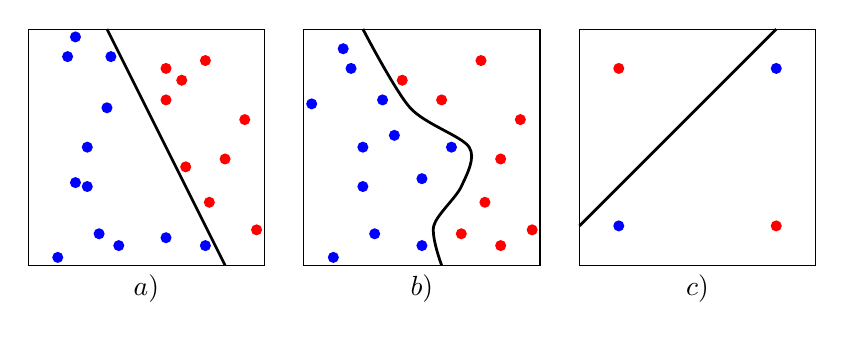
\begin{tikzpicture}[scale=0.5]
        % linearly separable box
        \draw (0,0) rectangle (6,6);
        \draw[text=black] (3,0) node[below] {$a)$};
        \draw[color=black,line width=1pt]
            (2,6) -- (5,0);

        % nonlinearly separable box
        \draw (7,0) rectangle (13,6);
        \draw[text=black] (10,0) node[below] {$b)$};
        \draw[color=black,line width=1pt] plot [smooth] coordinates {
            (8.5, 6) (9.7, 4) (11.2, 3) (11, 2) (10.3, 1) (10.5,0)};

        % XOR
        \draw (14,0) rectangle (20,6);
        \draw[text=black] (17,0) node[below] {$c)$};
        \draw[color=black,line width=1pt]
            (14,1) -- (19,6);

        \def\positive{{%
        % linear
        {.75, 0.2},
        {2.3, 0.5},
        {4.5, 0.5},
        {3.5, 0.7},
        {1.8, 0.8},
        {1.5, 2},
        {1.2, 2.1},
        {1.5, 3},
        {2, 4},
        {2.1, 5.3},
        {1, 5.3},
        {1.2, 5.8},
        % nonlinear
        {7.75, 0.2},
        {10, 0.5},
        {8.8, 0.8},
        {8.5, 2},
        {10, 2.2},
        {10.75, 3},
        {8.5, 3},
        {9.3, 3.3},
        {7.2, 4.1},
        {9, 4.2},
        {8.2, 5},
        {8, 5.5},
        % XOR
        {15, 1},
        {19, 5},
        }}

        % \draw positive dots
        \foreach \i in {0,...,25} {
          \pgfmathparse{\positive[\i][0]}\let \x \pgfmathresult;
          \pgfmathparse{\positive[\i][1]}\let \y \pgfmathresult;
          \fill[blue] (\x,\y) circle (4pt);
        }

        \def\negative{{%
        % linear
        {5.8, 0.9},
        {4.6, 1.6},
        {4, 2.5},
        {5, 2.7},
        {5.5, 3.7},
        {3.5, 4.2},
        {3.9, 4.7},
        {3.5, 5},
        {4.5, 5.2},
        % nonlinear
        {12, 0.5},
        {11, 0.8},
        {12.8, 0.9},
        {11.6, 1.6},
        {12, 2.7},
        {12.5, 3.7},
        {10.5, 4.2},
        {9.5, 4.7},
        {11.5, 5.2},
        % XOR
        {19, 1},
        {15, 5},
        }}

        % \draw negative dots
        \foreach \i in {0,...,19} {
          \pgfmathparse{\negative[\i][0]}\let \x \pgfmathresult;
          \pgfmathparse{\negative[\i][1]}\let \y \pgfmathresult;
          \fill[red] (\x,\y) circle (4pt);
        }
    \end{tikzpicture}
    \caption{a) A linearly separable problem. b) A nonlinearly separable
        problem. c) The XOR problem with a tentative solution that fails at
        separating the points of the space.\label{fig:XOR}}
\end{figure}

The excessive enthusiasm for the early successes of ANNs turned into strong
disappointment: even if~\cite{Minsky69} showed that an MLP could model the XOR
bitwise operation, they also pointed out that Rosenblatt's learning algorithm
was limited to single layered Perceptrons and could not autonomously learn how
to solve the problem. The expectation of an artificial intelligence that could
learn by itself to solve problems and interact with humans appeared suddenly
unrealistic and most of the research community lost interest in ANNs. The field
experienced a severe slow down and most of the fundings were cut.

After a decade known as the first AI Winter, in 1982 John Hopfield presented a
model of human memory that did not only give insights on how the brain works,
but was also useful in practical applications and had a sound and detailed
mathematical grounding. At the same time, at the US-Japan Joint Conference on
Cooperative/Competitive Neural Networks, Japan announced a renewed effort in
building neural networks and the fear that the US might be left behind renewed
their effort on this topic.

The breakthrough that completely restored the interest in the field came in
1986, when~\cite{Rumelhart86b} rediscovered the backpropagation
algorithm~\citep{Linnainmaa70,Werbos74} that allowed to train ANNs composed by
multiple layers by performing gradient descent~(see \autoref{sec:backprop}).
However once again the expectation was set too high and AI was expected to
allow to do things like translating languages, carring on conversations and
interpreting pictures. In late 80s and early 90s AI fundings were cut again
when those very high demands had not been attended.

Despite that, many researcher were convinced by then of the potential of AI
and kept working on it. By 2006 ANNs established the state of the art in many
official international competitions in several domains, attracting again
attention and fundings. Since then, they have been constantly the focus of
study and innovation.

\subsection{MultiLayer Perceptron}\label{sec:MLP}
\begin{figure}[t]
    \centering
    \begin{neuralnetwork} [nodespacing=7.5mm, layerspacing=23mm,
            maintitleheight=2.5em, layertitleheight=5em,
            height=3, toprow=true, nodesize=17pt,
            style={}, title={}, titlestyle={}]
        %%%%% Layers
        \inputlayer[count=2, bias=false, title=Input\\layer, text=\nodetextxi]
        \hiddenlayer[count=3, bias=true, title=Layer 1, text=\nodetexthi]
        {\setdefaultlinklabel{\wijllink}\linklayers}
        \hiddenlayer[count=5, bias=true, title=Layer 2, text=\nodetexthi]
        {\setdefaultlinklabel{\wijllink}\linklayers}
        \hiddenlayer[count=4, bias=true, title=Layer 3, text=\nodetexthi]
        {\setdefaultlinklabel{\wijllink}\linklayers}
        %\outputlayer[count=1, text=\nodetextsigma]
        %{\setdefaultlinklabel{\wijllink}\linklayers}
        %\redefinelayerspacing{20.5mm}
        %\outputlayer[count=1, text=\nodetextsigmoid]
        %\linklayers
        %\redefinelayerspacing{18.8mm}
        \outputlayer[count=1, text=\nodetexty]
        {\setdefaultlinklabel{\wijllink}\linklayers}
    \end{neuralnetwork}
    \centering
    \caption{\label{fig:MLP}A MultiLayer Perceptron. The sum and the
        nonlinearity nodes have been omitted for the sake of clarity.
    }
\end{figure}

\noindent Consider the network in~\autoref{fig:MLP}. As opposed to the
Perceptron in~\autoref{fig:perceptron}, the MLP has multiple hidden layers,
where each neuron of one hidden layer is connected to all the neurons of the
previous and the next layer. Each connection from the $i$-th neuron of layer
$l-1$ to the $j$-th neuron of layer $l$ is associated to a weight
$w_{ij}^{(l)}$, and all the weights are stored in a matrix $\mathbf{W^{(l)}}$.

Similarly to the Perceptron case, each layer computes an affine transformation

\begin{equation}\label{eq:MLP_affine}
    \mathbf{z}^{(l)} = \mathbf{W}^{(l)} \cdot \mathbf{a}^{(l-1)},
\end{equation}

\noindent followed by a nonlinearity $\sigma$ -- usually more smooth than the
one used in the Perceptron -- called \emph{activation function}

\begin{equation}\label{eq:MLP_activation}
    \mathbf{a}^{(l)} = \sigma(\mathbf{z}^{(l)}).
\end{equation}

One hidden layer can thus be seen as a function $h^{(l)}$ that depends on some
\emph{parameters} specific to that layer -- namely a matrix of weights
$\mathbf{w}^{(l)}$ and the bias vector $b^{(l)}$ -- as well as some
\emph{hyperparameters}, such as the number of neurons and the choice of
activation function. It is common to denote the set of trainable parameters
that fully characterize a layer as $\boldsymbol{\theta^{(l)}}$.

The processing performed by the hierarchy of layers of the MLP results in the
output vector $\mathbf{y}$ and is equivalent to a composition of multiple
functions

\begin{equation}\label{eq:fn_composition}
    \textbf{y} = h^{(L)}_{\boldsymbol{\theta}} \composition
        h^{(L-1)}_{\boldsymbol{\theta}} \composition
        \dots \composition h^{(1)}_{\boldsymbol{\theta}}.
\end{equation}

\noindent Although very common and widely used, the MLP is not the only
architecture for ANNs. In \autoref{sec:cnn} and \autoref{sec:rnn} two of the
most used alternatives will be described.

Generally, each layer of an ANN computes some activation based on its input and
a nonlinear activation function. The choice of which activation function to use
in each layer can have a big impact on the performance of the model and is
sometimes constrained by the semantic assigned to the output of some units. The
most important activation functions will be introduced in the following
section.

\subsection{Activation functions}\label{sec:activations}
\begin{figure}[t]
    \centering
    \begin{tikzpicture}[domain=-2.9:2.9]
        % grid
        \draw[very thin,color=gray] (-2.9, -1.1) grid (2.9, 2.9);
        \foreach \x in {-2,-1,0,1,2}
            \node[anchor=north] at (\x,-1.1) {\x};
        \foreach \y in {-1,0,1,2}
            \node[anchor=east] at (-2.9,\y) {\y};
        % axes
        \draw[->,thick] (-2.9, 0) -- (3.1, 0) node[right] {$z$};
        \draw[->,thick] (0, -1.1) -- (0, 3.1) node[above] {$f(z)$};

        % Logistic
        \draw[thick, color=blue]
            plot (\x, { 1/(1+exp(-1 * \x)) })
            node[right,yshift=-0.5em] {$logistic(z)$};
        % Beta logistic
        %\draw[color=purple] plot (\x, { 1/(1+exp(-.5 * \x)) })
        %    node[right] {$logistic(a), beta=.5$};
        % Tanh
        \draw[thick, color=orange]
            plot (\x, { ( 1 - exp(-2*\x) ) / ( 1 + exp(-2*\x) ) })
            node[right,yshift=0.5em] {$tanh(z)$};
        % ReLU
        \draw[thick, color=red]
            plot (\x, { max(0, \x) })
            %node[right] {$ReLU(x)$};
            node[xshift=-19.3em,yshift=-8em] (a) {$ReLU(z)$};
        % Leaky ReLU
        \draw[thick, color=yellow]
            plot (\x, { max(0.03 * \x, \x) })
            node[below = 1.2em of a.east, anchor=east] {$Leaky ReLU(z)$};
    \end{tikzpicture}
    \caption{Some of the most common activation functions: sigmoid, tanh, ReLU
        and Leaky ReLU. ReLU and Leaky ReLU are overlapping for $z \geq 0$.
        Best viewed in colors.\label{fig:activations}}
\end{figure}

The activation function is one of the most important component of an ANN. As
explained in the previous sections, to tackle nonlinearly separable problems it
is imperative to map the input into a space that is linearly separable. The
activation function does this by performing an \emph{element-wise nonlinear
transformation} of the pre-activation that comes from the affine
transformation.

The affine transformation and the nonlinearity work together in a very tight
interaction: the latter is fixed and does not evolve during training, but
maps its input to a different space in a (usually highly) non-linear way; the
former, is determined by the weights that are learned during training and
exploits the latter to map the incoming activation into a new space where they
are easier to separate. In addition to this it is interesting to point out that
if there was no activation function, since the composition of multiple affine
transformation is an affine transformation, the layers of the MLP could be
replaced by a single equivalent layer, and the MLP would become a Perceptron.

Many activation functions have been proposed in the years and even if our
understanding of this component has improved, which one to use with the
different architectures and tasks is still the object of active research.

\subsubsection{Logistic}\label{sec:logistic}
The logistic, often called \emph{sigmoid}, is a differentiable monotonically
increasing function that takes any real-valued number and maps it to $[0, 1]$.
As evident from its representation in~\autoref{fig:activations}, for large
negative numbers it asymptotes to $0$ while for large positive numbers it
asymptotes to $1$. It is defined as

\begin{equation}\label{eq:logistic}
    logistic(\mathbf{z}) = \frac{1}{1+\exp(-\mathbf{z})}.
\end{equation}

\noindent The logistic function has probably been the most used nonlinearity
historically due to its possible interpretation as the firing rate of a neuron,
or its probability to fire, given its potential (i.e., the level of excitement
provoked by its incoming spikes): when the potential is low the neuron fires
less often whereas when the potential is high the frequency of the spikes
increases.

Another very important property of the logistic function is that it is very
fast to compute its derivative, once solved analytically:

\begin{align}\label{eq:logistic_derivative}
\begin{split}% to show one label only
    \frac{\partial}{\partial \mathbf{z}}logistic(\mathbf{z}) &=
        \frac{\exp(\mathbf{-z})}{\left(1+\exp(-\mathbf{z})\right)^2} \\
    &= \frac{1}{1+\exp(-\mathbf{z})} \cdot
        \frac{\exp(-\mathbf{z})}{1+\exp(-\mathbf{z})} \\
    &= logistic(\mathbf{z}) \cdot
        \frac{\exp(-\mathbf{z})}{1+\exp(-\mathbf{z})} \\
    &= logistic(\mathbf{z}) \cdot
        \frac{1+\exp(-\mathbf{z})-1}{1+\exp(-\mathbf{z})} \\
    &= logistic(\mathbf{z}) \cdot
        \left(1-\frac{1}{1+\exp(-\mathbf{z})}\right) \\
    &= logistic(\mathbf{z}) \cdot (1-logistic(\mathbf{z}))
\end{split}
\end{align}

The use of the logistic function is not as widespread as it used to be though,
due to two major drawbacks:
\begin{itemize}
    \item \emph{Saturation kills the gradient:}
        backpropagation~(see~\autoref{sec:backprop}) relies on the gradient of
        the error to determine the parameters update. The logistic function
        saturates at both ends, resulting in a very small or zero gradient.
        This problem -- often referred to as~\emph{vanishing gradient} -- makes
        training very slow or prevents it in some cases. This also makes the
        logistic units very sensitive to the initialization of the weights of
        the network, that ideally should be such that the initial input of the
        logistic function is close to zero.
    \item \emph{The output is not zero-centered:} the dynamics of ANNs are
        usually complex and difficult to inspect, but it is widely believed
        that normalizing the intermediate activations of the network (i.e., to
        zero-center their mean and impose unit variance) helps
        training~\citep{Ioffe+Szegedy-2015,Laurent2015,arpit2016normalization,
        cooijmans2016recurrent}. The output of the logistic function is always
        positive, which causes the mean activation to be non-zero. This could
        introduce undesirable dynamics that could slow down or prevent
        training.
\end{itemize}

\subsubsection{Hyperbolic tangent (tanh)}\label{sec:tanh}

The hyperbolic tangent, typically shortened as~\emph{tanh}, is a differentiable
monotonically increasing function that maps any real-valued number to $[-1, 1]$.
This nonlinear function suffers from the same vanishing problem as the
logistic, but its mean is centered in zero. Furthermore, the tanh is often
chosen where it is desirable to be able to increase or decrease some quantity
by small amounts, thanks to its codomain. It is defined as

\begin{equation}\label{eq:tanh}
    tanh(\mathbf{z}) = \frac{1-exp(-2\mathbf{z})}{1+exp(-2\mathbf{z})}.
\end{equation}


\subsubsection{Rectified Linear Unit (ReLU)}\label{sec:relu}
Since its introduction, the Rectified Linear Unit
(ReLu)~\citep{Jarrett-ICCV2009-small,Nair+Hinton-2010} has become the
nonlinearity of choice in many applications~\citep{Krizhevsky-2012,
LeCun-et-al-Nature2015,Glorot+al-AI-2011-small}. It is defined as

\begin{equation}\label{eq:relu}
    relu(\mathbf{z}) = max(0, \mathbf{z}).
\end{equation}

Although very simple, it has some very interesting properties and only a few
drawbacks:

\begin{itemize}
    \item \emph{No positive saturation:} the ReLU is zero for non-positive
        inputs, but does not saturate otherwise. This ensures a flow of
        gradient whenever the input is positive, that was found to
        significantly speed up the convergence of training.
    \item \emph{Cheap to compute:} as opposed to many other activation
        functions that require expensive operations, such as for instance
        exponentials, ReLU's implementation simply amounts to thresholding at
        zero. Another important characteristic is that the gradient is trivial
        to compute:

        \begin{equation}\label{eq:relu_derivative}
            \nabla (relu(\mathbf{z}^{(l)})) =
                \begin{cases}
                    \mathbf{a}^{(l-1)},  & \text{if } \mathbf{z}^{(l)} > 0 \\
                    0,          & \text{if } \mathbf{z}^{(l)} < 0 \\
                    undefined,  & \text{if } \mathbf{z}^{(l)} = 0.
                \end{cases}
        \end{equation}

    \item \emph{Induce sparsity:} ReLU units induce sparsity, indeed whenever
        the input preactivation is negative their activation is zero. Sparsity
        is usually a desired property: as opposed to dense encoding, sparsity
        will produce representations where only a few entries change upon small
        variations of the input, i.e., it will produce a representation that is
        more consistent and robust to perturbations. Furthermore, sparsity
        allows for a more compact encoding, which is desirable in many contexts
        such as, e.g., data compression and efficient data transfer.  Finally,
        it is also usually easier to linearly separate sparse
        representations~\citep{Glorot+al-AI-2011-small}.
    \item \emph{ReLU units can die:} when a large gradient flows through a ReLU
        unit it can change its weights in such a way that will prevent it from
        ever being active again. In this case every input will put the ReLU
        unit on the flat zero side. This will prevent any gradient flow and the
        unit will never leave this state becoming \emph{de~facto} "dead". This
        can be alleviated by using a lower learning rate or choosing some
        modification of ReLU less sensitive to this problem.
\end{itemize}

\subsubsection{Leaky Rectified Linear Unit (Leaky ReLU)}\label{sec:lrelu}
Leaky ReLUs are one of the most adopted alternatives to ReLUs. They have been
proposed as a way to alleviate the dying units problem of ReLUs, by preventing
the unit from saturating thus allowing a small gradient to always flow through
the unit, potentially recovering extreme values of the weights. Leaky ReLUs are
defined as

\begin{equation}\label{eq:lrelu}
    leaky\_relu(\mathbf{z}) = max(\beta*\mathbf{z}, \mathbf{z}),
\end{equation}

\noindent where $\beta$ is a small constant.

\subsubsection{Softmax}\label{sec:softmax}
One peculiar nonlinearity that deserves a particular mention is the softmax.
This function differs from the previously described activations in that it
does not only depend on the value of the preactivation in one dimension (i.e.,
the value of one unit), but rather on the preactivation in all the dimensions
altogether. The softmax is a \emph{squashing~function} that maps its input to a
categorical distribution. It is defined as

\begin{equation}\label{eq:softmax}
    softmax(z_i) = \frac{\exp(z_i)}{\sum_{k=0}^K{\exp(z_k)}},
\end{equation}

\noindent where $K$ is the number of classes, i.e., of dimensions (or neurons).

Note that it is possible to add a temperature parameter $T$ to the softmax that
allows it to control its steepness (see~\autoref{fig:softmax}), i.e., to
control the randomness of predictions. When $T$ is high the distribution over
the classes will be more uniform - with the extreme case of $T = \inf$, where
all the classes have equal probability. When $T$ is low, the probability curve
is more peacky on the class with higher probability and has a light tail on the
other classes.

\begin{equation}\label{eq:softmax_tmp}
    softmax(z_i) = \frac{\exp(z_i / T)}
                        {\sum_{k=0}^K{\exp(z_k / T)}}.
\end{equation}

\begin{figure}[t]
    \centering
    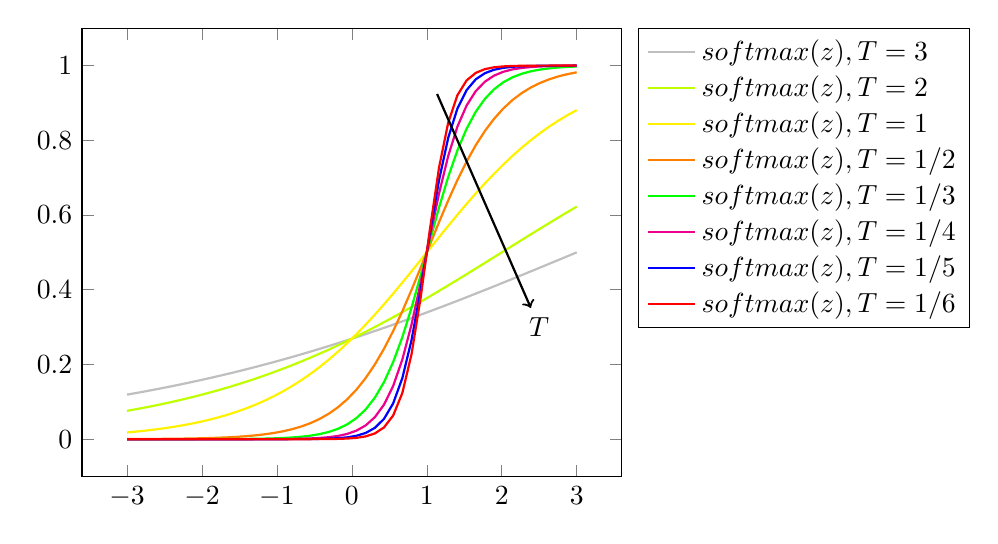
\begin{tikzpicture}
        % grid
        % \draw[very thin,color=gray] (-4.1, -1.1) grid (4.1, 1.1);
        % \foreach \x in {-4,-3,-2,-1,0,1,2,3,4}
        %     \node[anchor=north] at (\x,-1) {\x};
        % \foreach \y in {-1,0,1}
        %     \node[anchor=east] at (-1,\y) {\y};
        % axes
        %\draw[->,thick] (-4.1, 0) -- (4.1, 0) node[right] {$x$};
        %\draw[->,thick] (0, -1.1) -- (0, 1.1) node[above] {$f(x)$};

        % softmax
        \begin{axis}[samples=50,
                     domain=-3:3,
                     restrict y to domain =-20:100,
                     legend cell align=left,
                     legend pos=outer north east,
                     %legend style={draw=none}
                 ]
            \addplot[thick,lightgray]plot (\x, { exp(\x/3)/(exp(1) + exp(\x / 3)) });
            \addplot[thick,lime     ]plot (\x, { exp(\x/2)/(exp(1) + exp(\x / 2)) });
            \addplot[thick,yellow   ]plot (\x, { exp(1 * \x)/(exp(1) + exp(1 * \x)) });
            \addplot[thick,orange   ]plot (\x, { exp(2 * \x)/(exp(2) + exp(2 * \x)) });
            \addplot[thick,green    ]plot (\x, { exp(3 * \x)/(exp(3) + exp(3 * \x)) });
            \addplot[thick,magenta  ]plot (\x, { exp(4 * \x)/(exp(4) + exp(4 * \x)) });
            \addplot[thick,blue     ]plot (\x, { exp(5 * \x)/(exp(5) + exp(5 * \x)) });
            \addplot[thick,red      ]plot (\x, { exp(6 * \x)/(exp(6) + exp(6 * \x)) });
            \node[anchor=west] (source) at (axis cs:0.95,0.95){};
            \node (destination) at (axis cs:2.5,0.3){$T$};
            \draw[thick, ->](source)--(destination);

            \addlegendentry{$softmax(z), T= 3$}
            \addlegendentry{$softmax(z), T= 2$}
            \addlegendentry{$softmax(z), T= 1$}
            \addlegendentry{$softmax(z), T= 1/2$}
            \addlegendentry{$softmax(z), T= 1/3$}
            \addlegendentry{$softmax(z), T= 1/4$}
            \addlegendentry{$softmax(z), T= 1/5$}
            \addlegendentry{$softmax(z), T= 1/6$}
        \end{axis}
    \end{tikzpicture}
    \caption{The behaviour of softmax as temperature $T$ grows. The plots have
        been obtained considering a bidimensional input setting where the
        preactivation associated to the second class $z_1$ is always $1$. As
        $T$ decreases, the function becomes steeper.\label{fig:softmax}}
\end{figure}

\subsection{Backpropagation}\label{sec:backprop}
The learning rule originally introduced with Perceptrons did not allow one to
train models with multiple layers (i.e., with \emph{hidden} layers), such as
the one depicted in~\autoref{fig:MLP}.

This was not possible since to compute the variation of the weights of a layer
with~\autoref{eq:perceptron_lr} it is necessary to know the correct value of
its output, which is given only for the last layer.

To address this obstacle it suffices to notice that the computation performed
by each activation function is a nonlinear, but differentiable function of the
inputs. This allows for the computation of the partial derivatives of the error
(e.g., the expected value of the quadratic loss) with respect to the weights of
the network. In other words, it is possible to use calculus to determine the
amount by which each neuron of the last layer contributed to causing the error,
and then further split the responsibility of each of them among the ones of the
preceding layer. In this way, the error can be \emph{backpropagated} through
the layers of the network, assigning to each weight its amount of blame. This
information can be used by an \emph{optimization algorithm} to iteratively
change the weights to minimize the error.

The backpropagation algorithm has some resemblance with the learning rule of
the Perceptron~(\autoref{eq:perceptron_lr}). The main idea in that case was
to modify each weight of the network by a factor proportional to the error
($E = \hat y - y$, in the Perceptron) and to the input. Even if in MLPs it is
usually common to consider different kinds of cost functions, the same concept
applies: the learning procedure tries to modify the weights in order to
minimize some error

\begin{equation}
    %w_{ij}^{(l)} = w_{ij}^{(l)} + \eta \frac{\partial E}{\partial w_{ij}^{(l)}}
    \mathbf{W} = \mathbf{W} - \eta \frac{\partial E}{\partial \mathbf{W}},
\end{equation}

\noindent where $\eta$ is a scaling factor typically referred to as
\emph{learning rate}, that determines the size of the gradient descent steps.

It is easier to understand backpropagation with a practical example. Consider
once again~\autoref{fig:MLP}: the network processes a bidimensional input
$\mathbf{x}$ and, after three layers of affine transformations followed by
nonlinearities, returns a unidimensional value $\mathbf{\hat y}$. The correct
output $\mathbf{y}$ is given and is used to compute the error, or~\emph{cost},
with some \emph{differentiable} metric. For this example consider the mean
squared error (MSE)

\begin{equation}\label{eq:MSE}
    E_{mse} = \frac{1}{M} \sum_{\mathcal{D}}\frac{1}{2}(\mathbf{y} - \mathbf{\hat y})^2,
\end{equation}

\noindent the summation is done over a dataset $\mathcal{D}$ of $M$ samples,
each composed by an input $\mathbf{x}$ and its associated desired output
$\mathbf{y}$. $\mathbf{\hat y}$ is used as a compact notation for
$\mathbf{\hat y(x)}$ and represents the output of the network for one input sample
$\mathbf{x}$.

It is possible to compute the fraction of the error that can be attributed to
each neuron of the network by taking the derivative of the error with respect
to it

\begin{align}\label{eq:backprop_step1}
\begin{split}
    \frac{\partial E_{mse}}{\partial w_{ij}^{(l)}} &=
    \frac{\partial}{\partial w_{ij}^{(l)}}\left(
        \frac{1}{m}\sum_{\mathcal{D}}\left[
        \frac{1}{2}(\mathbf{y} - \mathbf{\hat y})^2\right]\right) \\
    &= \frac{1}{m}\sum_{\mathcal{D}} \left[\frac{1}{2}
        \frac{\partial}{\partial w_{ij}^{(l)}}
        \left(\mathbf{y} - \mathbf{\hat y}\right)^2\right] \\
    &= \frac{1}{m}\sum_{\mathcal{D}}\left[(\mathbf{y} - \mathbf{\hat y})
        \cdot \frac{\partial}{\partial w_{ij}^{(l)}}(-\mathbf{\hat y})\right] \\
\end{split}
\end{align}

Backpropagation allows one to compute the partial derivative
$\frac{\partial}{\partial w_{ij}^{(l)}}(-\mathbf{\hat y})$
exploiting the chain rule of derivation. Consider e.g., the weights of the
second layer $\mathbf{W}^{(2)}$

\begin{align}\label{eq:backprop_step2}
\begin{split}
    -\frac{\partial\mathbf{\hat y}}{\partial \mathbf{W}^{(2)}} &=
        -\frac{\partial \mathbf{\hat y}}{\partial \mathbf{z}^{(4)}} \cdot
        \frac{\partial \mathbf{z}^{(4)}}{\partial \mathbf{W}^{(2)}} \\
    &= -\frac{\partial \mathbf{\hat y}} {\partial \mathbf{z}^{(4)}} \cdot
        \frac{\partial \mathbf{z}^{(4)}}{\partial \mathbf{a}^{(3)}} \cdot
        \frac{\partial \mathbf{a}^{(3)}}{\partial \mathbf{W}^{(2)}} \\
    &= -\frac{\partial \mathbf{\hat y}} {\partial \mathbf{z}^{(4)}} \cdot
        \frac{\partial \mathbf{z}^{(4)}}{\partial \mathbf{a}^{(3)}} \cdot
        \frac{\partial \mathbf{a}^{(3)}}{\partial \mathbf{z}^{(3)}} \cdot
        \frac{\partial \mathbf{z}^{(3)}}{\partial \mathbf{W}^{(2)}} \\
    &= -\frac{\partial \mathbf{\hat y}} {\partial \mathbf{z}^{(4)}} \cdot
        \frac{\partial \mathbf{z}^{(4)}}{\partial \mathbf{a}^{(3)}} \cdot
        \frac{\partial \mathbf{a}^{(3)}}{\partial \mathbf{z}^{(3)}} \cdot
        \frac{\partial \mathbf{z}^{(3)}}{\partial \mathbf{a}^{(2)}} \cdot
        \frac{\partial \mathbf{a}^{(2)}}{\partial \mathbf{W}^{(2)}} \\
    &= -\frac{\partial \mathbf{\hat y}} {\partial \mathbf{z}^{(4)}} \cdot
        \frac{\partial \mathbf{z}^{(4)}}{\partial \mathbf{a}^{(3)}} \cdot
        \frac{\partial \mathbf{a}^{(3)}}{\partial \mathbf{z}^{(3)}} \cdot
        \frac{\partial \mathbf{z}^{(3)}}{\partial \mathbf{a}^{(2)}} \cdot
        \frac{\partial \mathbf{a}^{(2)}}{\partial \mathbf{z}^{(2)}} \cdot
        \frac{\partial \mathbf{z}^{(2)}}{\partial \mathbf{W}^{(2)}}
\end{split}
\end{align}

\noindent Since $\partial\sigma(\mathbf{a})=\sigma' \hadamard
\partial\mathbf{a}$, from \autoref{eq:MLP_affine} and
\autoref{eq:MLP_activation} follows

\begin{equation}\label{eq:backprop_step3}
    -\frac{\partial\mathbf{\hat y}}{\partial \mathbf{W}^{(2)}} =
        \sigma'(\mathbf{z}^{(4)}) \hadamard \mathbf{W}^{(4)} \cdot
        \sigma'(\mathbf{z}^{(3)}) \hadamard \mathbf{W}^{(3)} \cdot
        \sigma'(\mathbf{z}^{(2)}) \hadamard \mathbf{a}^{(1)^T},
\end{equation}

\noindent where $\mathbf{a} \hadamard \mathbf{b}$ represents the elementwise
product of two vectors $\mathbf{a}$ and $\mathbf{b}$, also known as the
Hadamard product. By applying the rule $\mathbf{A} \cdot (\mathbf{B} \hadamard
\mathbf{C}) = (\mathbf{A} \hadamard \mathbf{B}) \cdot \mathbf{C}$,
\autoref{eq:backprop_step3} can be rewritten as

\begin{equation}\label{eq:backprop_step4}
    -\frac{\partial\mathbf{\hat y}}{\partial \mathbf{W}^{(2)}} =
        \sigma'(\mathbf{z}^{(4)}) \hadamard \mathbf{W}^{(4)} \cdot
        \sigma'(\mathbf{z}^{(3)}) \hadamard \mathbf{W}^{(3)} \cdot
        \sigma'(\mathbf{z}^{(2)}) \hadamard \mathbf{a}^{(1)}.
\end{equation}

Note that $\sigma'$ can be computed analytically and depends on the activation
function of choice (see e.g.~\autoref{eq:logistic_derivative} and
\autoref{eq:relu_derivative}).

% The rest of this chapter will focus on two very common kinds of ANNs
% respectively characterized by a feedforward and feedback connectivity pattern,
% namely Convolutional Neural Networks and Recurrent Neural Networks.


%================================== SECTION ==================================
\section{Convolutional networks}\label{sec:cnn}

Deep CNNs have been at the heart of spectacular advances in deep learning.
Although CNNs have been used as early as the nineties to solve character
recognition tasks \citep{le1997reading}, their current popularity is due to
much more recent work, when a deep CNN was used to beat state-of-the-art in the
ImageNet image classification challenge~\citep{krizhevsky2012imagenet}.

% \begin{figure}[t] --> already in ReNet
%     \centering
%     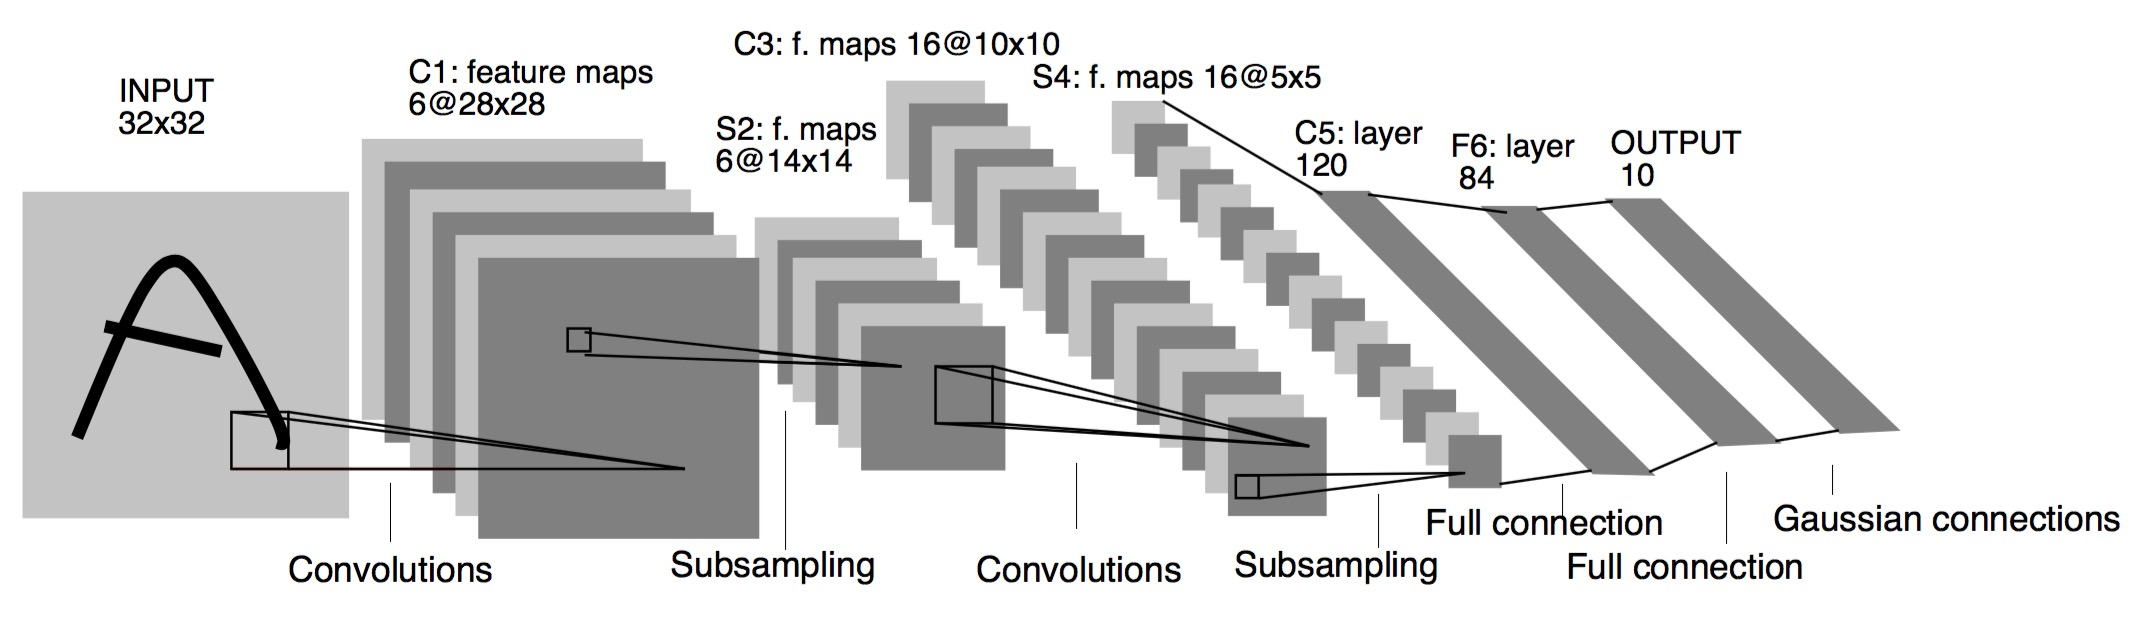
\includegraphics[width=0.8\textwidth]{img/renet/lenet5.jpg}
%     \caption{\label{fig:lenet} The LeNet architecture for handwritten
%         characters recognition.}
% \end{figure}
%
\autoref{sec:MLP} introduced MLPs, a powerful and very common ANN architecture
that computes at each layer an affine transformation of its inputs followed by
an activation function. One property of MLPs is that they are dense, in the
sense that they often connect all the units of one layer to all the units of
the next layer (often referred to as being \emph{fully connected}). When the
input has a structure, a dense connectivity pattern might be wasteful and it is
usually preferable to be able to exploit the data structure. The reason for
this is twofold: first, adapting the connectivity pattern to the structure of
the data reduces the number of parameters and of operations performed by the
network and, consequently, the memory usage and the computation time; second,
constraining the connectivity pattern can have the effect of forcing the
network to focus on what is important, yielding faster training and better
performance.

Convolutional neural networks (CNNs) are an example of models that exploit
the structure of the data. The intuition behind CNNs is that many kinds of data
-- such as images or audio clips -- have a \emph{local} topological structure
that does not depend on the specific location in the global reference system.
In the case of images, for example, this means that a hand can appear in the
center of the image as well as in one of the corners, and is not less of a hand
in either cases. Similarly, the sound of the word \emph{hand} should be
detected the same way when pronounced with a high or low pitch.

CNNs exploit this understanding of the data by applying the same pattern
detector at many locations in the image. This is formally done through a
\emph{convolution} (hence the name CNN), a signal processing operation that
superimposes a pattern detector -- usually called \emph{filter}, \emph{kernel}
or \emph{mask} -- on different locations of the image and emits an activation
in each position. In the previous example this would mean applying a "hand
detector" on every location of the image to produce a matrix of activations,
typically referred to as \emph{feature map}. In any real-world application
though, it would be common to apply multiple kernels at once with the same
convolution, hence obtaining a tensor of feature maps.

The convolution operation can be seen as the repetition of two operations: the
superimposition of one or more kernels in one position, followed by a shift --
or \emph{stride} -- of the kernels to allow their subsequent applications in
the next position. This system works successfully in most cases, but it would
most likely fail to e.g., detect hands that are not completely contained in the
image. The typical solution adopted to overcome this limitation is to
\emph{pad} the image by adding a frame (usually of zeros) around it on every
side. This ensures that on the borders of the image the convolution performs
both a complete superimposition of the kernel on every position in the image,
as well as partial ones (that is, a superimposition that is partially on the
image and partially on the padding).  In the padded half hand scenario, this
partial superimposition over the image would cause an activation that is not as
strong as in the case of a full overlap, but not zero either.

The elements described so far fully define a convolution. The shape of the
feature maps produced by a convolutional layer is affected by the shape of its
input as well as the choice of kernel shape, zero padding and strides, and the
relationship between these properties is not always trivial to infer. This
contrasts with fully-connected layers, whose output size is independent of the
input size.

Additionally, CNNs also usually feature {\em pooling\/} layers, adding yet
another level of complexity with respect to fully-connected networks. Finally,
so-called transposed convolutional layers (also known as fractionally strided
convolutional layers) have been employed in more and more work as of late
\citep{zeiler2011adaptive,zeiler2014visualizing,
long2015fully,radford2015unsupervised,Visin_2016_CVPR_Workshops,
im2016generating}, and their relationship with convolutional layers has been
explained with various degrees of clarity.

%Learning how to use CNNs for the first time can be an intimidating experience.
The convolution operation will be formally introduced
in~\autoref{sec:discrete_conv} followed by a description of pooling
in~\autoref{sec:pooling}. The rest of this section will focus on the arithmetic
to compute the output shape of a convolution given its parameters. In
particular~\autoref{sec:transposed_conv} targets transposed convolutions, a
smart application of convolutions to upsampling. For an in-depth treatment of
the subject, see Chapter 9 of the Deep Learning
textbook~\citep{Goodfellow-et-al-2016-Book}.

\subsection{Discrete convolutions}\label{sec:discrete_conv}

The bread and butter of neural networks is \emph{affine transformations}: a
vector is received as input and is multiplied with a matrix to produce an
output (to which a bias vector is usually added before passing the result
through a nonlinearity). This is applicable to any type of input, be it an
image, a sound clip or an unordered collection of features; whatever their
dimensionality, their representation can always be flattened into a vector
before the transformation.

Images, sound clips and many other similar kinds of data have an intrinsic
structure. More formally, they share these important properties:

\begin{itemize}
    \item They are stored as multi-dimensional arrays.
    \item They feature one or more axes for which ordering matters (e.g., width
        and height axes for an image, time axis for a sound clip, etc, ..).
    \item One axis, called the channel axis, is used to access different views
        of the data (e.g., the red, green and blue channels of a color image, or
        the left and right channels of a stereo audio track).
\end{itemize}

These properties are not exploited when an affine transformation is applied; in
fact, all the axes are treated in the same way and the topological information
is not taken into account. Still, taking advantage of the implicit structure of
the data may prove very handy in solving some tasks, like computer vision and
speech recognition, and in these cases it would be best to preserve it. This is
where discrete convolutions come into play.

A discrete convolution is a linear transformation that preserves this notion of
ordering. It is sparse (only a few input units contribute to a given output
unit) and reuses parameters (the same weights are applied to multiple locations
in the input). \autoref{fig:numerical_no_padding_no_strides} provides an
example of a discrete convolution. The light blue grid is called the {\em input
feature map}. To keep the drawing simple, a single input feature map is
represented, but it is not uncommon to have multiple feature maps stacked one
onto another.\footnote{An example of this is what was referred to earlier as
    {\em channels\/} for images and sound clips.}

A {\em kernel\/} (shaded area) with the following weights:

\begin{figure}[H]
    \centering
    \begin{tikzpicture}[scale=.4,every node/.style={minimum size=1cm}, on grid]
            \draw[fill=base02,opacity=0.4] (0,0) rectangle (3,3);
            \draw[draw=base03,thick] (0,0) grid (3,3);
            \node (00) at (0.5,2.5) {\tiny 0};
            \node (01) at (1.5,2.5) {\tiny 1};
            \node (02) at (2.5,2.5) {\tiny 2};
            \node (10) at (0.5,1.5) {\tiny 2};
            \node (11) at (1.5,1.5) {\tiny 2};
            \node (12) at (2.5,1.5) {\tiny 0};
            \node (20) at (0.5,0.5) {\tiny 0};
            \node (21) at (1.5,0.5) {\tiny 1};
            \node (22) at (2.5,0.5) {\tiny 2};
    \end{tikzpicture}
\end{figure}

\begin{figure}[p]
    \centering
    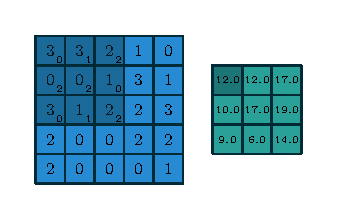
\includegraphics[width=0.32\textwidth]{pdf/numerical_no_padding_no_strides_00.pdf}
    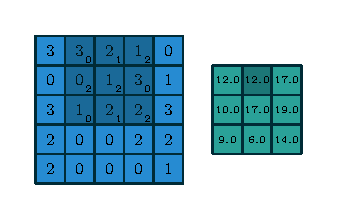
\includegraphics[width=0.32\textwidth]{pdf/numerical_no_padding_no_strides_01.pdf}
    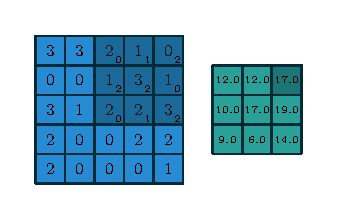
\includegraphics[width=0.32\textwidth]{pdf/numerical_no_padding_no_strides_02.pdf}
    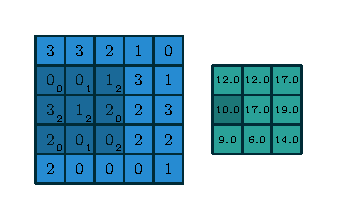
\includegraphics[width=0.32\textwidth]{pdf/numerical_no_padding_no_strides_03.pdf}
    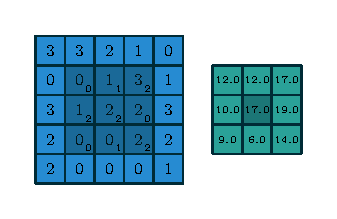
\includegraphics[width=0.32\textwidth]{pdf/numerical_no_padding_no_strides_04.pdf}
    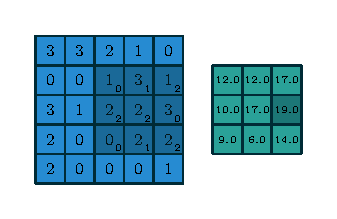
\includegraphics[width=0.32\textwidth]{pdf/numerical_no_padding_no_strides_05.pdf}
    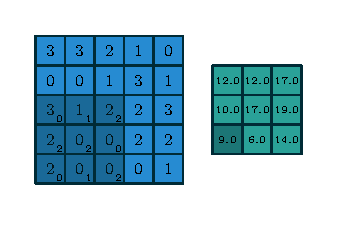
\includegraphics[width=0.32\textwidth]{pdf/numerical_no_padding_no_strides_06.pdf}
    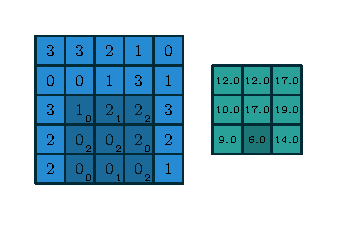
\includegraphics[width=0.32\textwidth]{pdf/numerical_no_padding_no_strides_07.pdf}
    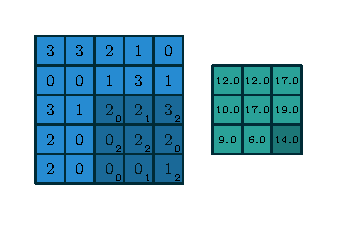
\includegraphics[width=0.32\textwidth]{pdf/numerical_no_padding_no_strides_08.pdf}
    \caption{\label{fig:numerical_no_padding_no_strides} Computing the output
        values of a discrete convolution.}
\end{figure}

\begin{figure}[p]
    \centering
    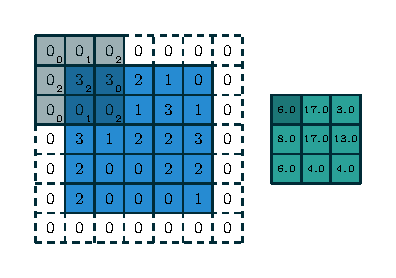
\includegraphics[width=0.32\textwidth]{pdf/numerical_padding_strides_00.pdf}
    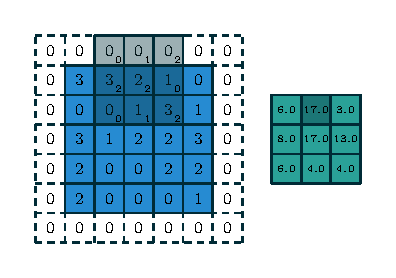
\includegraphics[width=0.32\textwidth]{pdf/numerical_padding_strides_01.pdf}
    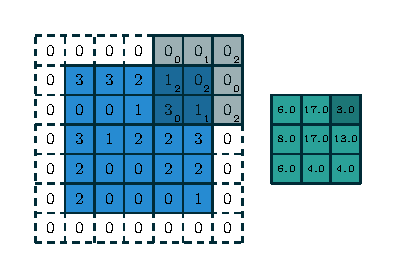
\includegraphics[width=0.32\textwidth]{pdf/numerical_padding_strides_02.pdf}
    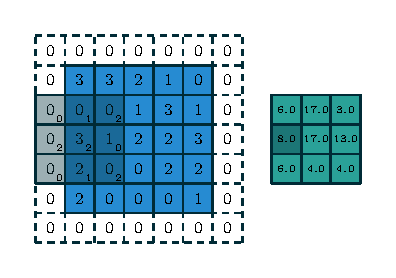
\includegraphics[width=0.32\textwidth]{pdf/numerical_padding_strides_03.pdf}
    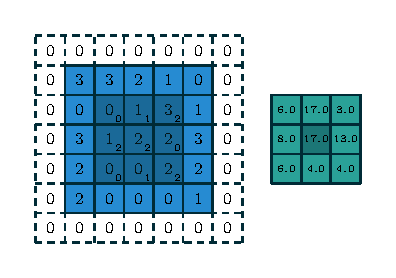
\includegraphics[width=0.32\textwidth]{pdf/numerical_padding_strides_04.pdf}
    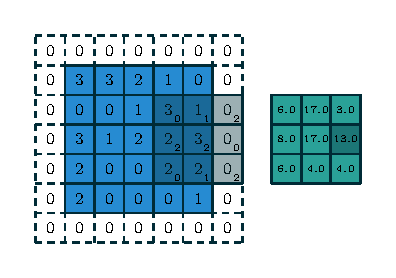
\includegraphics[width=0.32\textwidth]{pdf/numerical_padding_strides_05.pdf}
    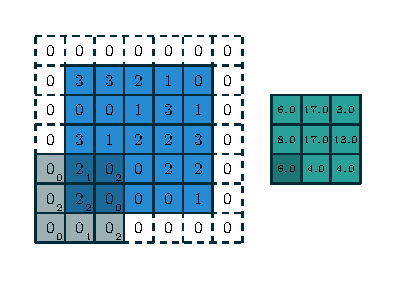
\includegraphics[width=0.32\textwidth]{pdf/numerical_padding_strides_06.pdf}
    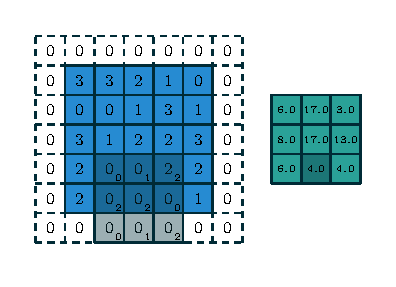
\includegraphics[width=0.32\textwidth]{pdf/numerical_padding_strides_07.pdf}
    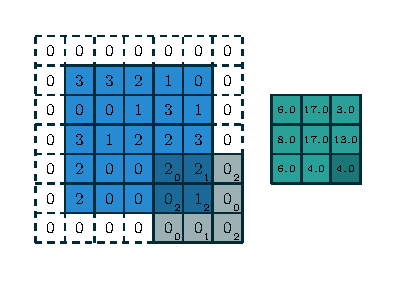
\includegraphics[width=0.32\textwidth]{pdf/numerical_padding_strides_08.pdf}
    \caption{\label{fig:numerical_padding_strides} Computing the output values
        of a discrete convolution for $N = 2$, $i_1 = i_2 = 5$, $k_1 = k_2 = 3$,
        $s_1 = s_2 = 2$, and $p_1 = p_2 = 1$.}
\end{figure}

\noindent slides across the input feature map. At each location, the product
between each element of the kernel and the input element it overlaps is computed
and the results are summed up to obtain the output in the current location. The
procedure can be repeated using different kernels to form as many output feature
maps as desired (\autoref{fig:full_picture}). The final outputs of this procedure
are called {\em output feature maps}.\footnote{%
    While there is a distinction between convolution and cross-correlation from
    a signal processing perspective, the two become interchangeable when the
    kernel is learned. For the sake of simplicity and to stay consistent with
    most of the machine learning literature, the term {\em convolution\/}
    will be used in this guide.}
If there are multiple input feature maps, the kernel will have to be
3-dimensional -- or, equivalently, each one of the feature maps will be
convolved with a distinct kernel -- and the resulting feature maps will
be summed up elementwise to produce the output feature map. The convolution
depicted in \autoref{fig:numerical_no_padding_no_strides} is an instance of a
2-D convolution, but it can be generalized to N-D convolutions.  For instance,
in a 3-D convolution, the kernel would be a {\em cuboid\/} and would slide
across the height, width and depth of the input feature map.

The collection of kernels defining a discrete convolution has a shape
corresponding to some assignment of $(n, m, k_1, \ldots, k_N)$, where

\begin{equation*}
\begin{split}
    n &\equiv \text{number of output feature maps},\\
    m &\equiv \text{number of input feature maps},\\
    k_j &\equiv \text{kernel size along axis $j$}.
\end{split}
\end{equation*}

The following properties affect the output size $o_j$ of a convolutional layer
along axis $j$:

\begin{itemize}
    \item $i_j$: input size along axis $j$,
    \item $k_j$: kernel size along axis $j$,
    \item $s_j$: stride (distance between two consecutive positions of the
        kernel) along axis $j$,
    \item $p_j$: zero padding (number of zeros concatenated at the beginning and
        at the end of an axis) along axis $j$.
\end{itemize}

\noindent For instance, \autoref{fig:numerical_padding_strides} shows a $3
\times 3$ kernel applied to a $5 \times 5$ input padded with a $1 \times 1$
border of zeros using $2 \times 2$ strides.

Note that strides constitute a form of \emph{subsampling}. As an alternative to
being interpreted as a measure of how much the kernel is translated, strides
can also be viewed as how much of the output is retained. For instance, moving
the kernel by hops of two is equivalent to moving the kernel by hops of one but
retaining only odd output elements (\autoref{fig:strides_subsampling}).

\begin{figure}[p]
    \centering
    \begin{tikzpicture}[scale=.35,every node/.style={minimum size=1cm}, on grid]
        \begin{scope}[xshift=0cm,yshift=0cm]
            \begin{scope}[xshift=0cm,yshift=0cm]
                \draw[draw=base03,fill=violet,thick]
                    (0,0) grid (5,5) rectangle (0,0);
            \end{scope}
            \begin{scope}[xshift=0.5cm,yshift=0.5cm]
                \draw[draw=base03,fill=blue,thick]
                    (0,0) grid (5,5) rectangle (0,0);
            \end{scope}
        \end{scope}
        \foreach \x in {-10,1,11} {%
            \begin{scope}[xshift=\x cm,yshift=10cm]
                \begin{scope}[xshift=0cm,yshift=0cm]
                    \draw[draw=base03,fill=violet,thick]
                        (0,0) grid (3,3) rectangle (0,0);
                \end{scope}
                \begin{scope}[xshift=0.5cm,yshift=0.5cm]
                    \draw[draw=base03,fill=blue,thick]
                        (0,0) grid (3,3) rectangle (0,0);
                \end{scope}
            \end{scope}
            \begin{scope}[xshift=\x cm,yshift=20cm]\begin{scope}[xshift=0.5cm]
                \draw[draw=base03,fill=cyan,thick]
                    (0,0) grid (3,3) rectangle (0,0);
            \end{scope}\end{scope}
        }
        \begin{scope}[xshift=1cm,yshift=30cm]
            \foreach \s in {0.0,0.5,1.0} {%
                \begin{scope}[xshift=\s cm,yshift=\s cm]
                    \draw[draw=base03,fill=cyan,thick]
                        (0,0) grid (3,3) rectangle (0,0);
                \end{scope}
            }
        \end{scope}
        \draw[->, thick] (-0.5,2.5) to (-8.5,9.5);
        \draw[->, thick] (3,6) to (3,9.5);
        \draw[->, thick] (6,3.5) to (12.5,9.5);
        \draw[thick]  (-8,14.5) to (-8,16);
        \draw[->, thick]  (-8,18) to (-8,19.5);
        \node[thick] (p1) at (-8,17) {$+$};
        \draw[thick]  (3,14.5) to (3,16);
        \draw[->, thick]  (3,18) to (3,19.5);
        \node[thick] (p2) at (3,17) {$+$};
        \draw[thick]  (13,14.5) to (13,16);
        \draw[->, thick]  (13,18) to (13,19.5);
        \node[thick] (p3) at (13,17) {$+$};
        \draw[->, thick]  (-8,23.5) to (2,29.5);
        \draw[->, thick]  (3,23.5) to (2.5,29.5);
        \draw[->, thick]  (13,23.5) to (3,29.5);
    \end{tikzpicture}
    \caption{\label{fig:full_picture} A convolution mapping from two input
        feature maps to three output feature maps using a $3 \times 2 \times 3
        \times 3$ collection of kernels $\mathbf{w}$. In the left pathway, input
        feature map 1 is convolved with kernel $\mathbf{w}_{1,1}$ and input
        feature map 2 is convolved with kernel $\mathbf{w}_{1,2}$, and the
        results are summed together elementwise to form the first output feature
        map. The same is repeated for the middle and right pathways to form the
        second and third feature maps, and all three output feature maps are
        grouped together to form the output.}
\end{figure}

\begin{figure}[p]
    \centering
    \begin{tikzpicture}[scale=.35,every node/.style={minimum size=1cm}, on grid]
        \begin{scope}[xshift=0,yshift=0cm]
            \begin{scope}[xshift=0cm,yshift=0cm]
                \draw[draw=base03,fill=blue,thick] (0,0) grid (5,5) rectangle (0,0);
                \draw[fill=base02, opacity=0.4] (0,2) rectangle (3,5);
            \end{scope}
            \begin{scope}[xshift=7cm,yshift=1.5cm]
                \draw[draw=base03,fill=cyan,thick] (0,0) grid (2,2) rectangle (0,0);
            \end{scope}
        \end{scope}
        \draw[draw=base03, ->, thick] (2.6,3.5) to  (4.5,3.5);
        \draw[draw=base03, ->, thick] (1.5,2.4) to (1.5,0.5);
        \draw[draw=base03, ->, thick] (5.25, 2.5) to (6.75, 2.5);
        \begin{scope}[xshift=12cm,yshift=0cm]
            \begin{scope}[xshift=0cm,yshift=0cm]
                \draw[draw=base03,fill=blue,thick] (0,0) grid (5,5) rectangle (0,0);
                \draw[fill=base02, opacity=0.4] (0,2) rectangle (3,5);
            \end{scope}
            \begin{scope}[xshift=7cm,yshift=1cm]
                \draw[draw=base03,fill=cyan,thick] (0,0) grid (3,3) rectangle (0,0);
                \draw[draw=base03] (1,0) -- (2,1) -- (2,0) -- (1,1);
                \draw[draw=base03] (0,1) -- (1,2) -- (1,1) -- (0,2);
                \draw[draw=base03] (1,1) -- (2,2) -- (2,1) -- (1,2);
                \draw[draw=base03] (2,1) -- (3,2) -- (3,1) -- (2,2);
                \draw[draw=base03] (1,2) -- (2,3) -- (2,2) -- (1,3);
            \end{scope}
            \begin{scope}[xshift=12cm,yshift=1.5cm]
                \draw[draw=base03,fill=cyan,thick] (0,0) grid (2,2) rectangle (0,0);
            \end{scope}
        \end{scope}
        \draw[draw=base03, ->, thick] (14.6,3.5) to  (15.5,3.5);
        \draw[draw=base03, ->, thick] (15.6,3.5) to  (16.5,3.5);
        \draw[draw=base03, ->, thick] (13.5,2.4) to (13.5,1.5);
        \draw[draw=base03, ->, thick] (13.5,1.4) to (13.5,0.5);
        \draw[draw=base03, ->, thick] (17.25, 2.5) to (18.75, 2.5);
        \draw[draw=base03, ->, thick] (22.25, 2.5) to (23.75, 2.5);
    \end{tikzpicture}
    \caption{\label{fig:strides_subsampling} An alternative way of viewing
        strides. Instead of translating the $3 \times 3$ kernel by increments of
        $s = 2$ (left), the kernel is translated by increments of $1$ and only
        one in $s = 2$ output elements is retained (right).}
\end{figure}

\subsection{Pooling}\label{sec:pooling}

In addition to discrete convolutions themselves, {\em pooling\/} operations
constitute another important building block in CNNs. Pooling operations reduce
the size of feature maps by using some function to summarize subregions, such
as taking the average or the maximum value.

Pooling works by sliding a window across the input and feeding the content of
the window to a {\em pooling function}. In some sense, pooling works very much
like a discrete convolution, but replaces the linear combination described by
the kernel with some other function. \autoref{fig:numerical_average_pooling}
provides an example for average pooling, and \autoref{fig:numerical_max_pooling}
does the same for max pooling.

The following properties affect the output size $o_j$ of a pooling layer
along axis $j$:

\begin{itemize}
    \item $i_j$: input size along axis $j$,
    \item $k_j$: pooling window size along axis $j$,
    \item $s_j$: stride (distance between two consecutive positions of the
        pooling window) along axis $j$.
\end{itemize}

\begin{figure}[p]
    \centering
    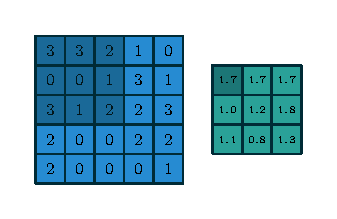
\includegraphics[width=0.32\textwidth]{pdf/numerical_average_pooling_00.pdf}
    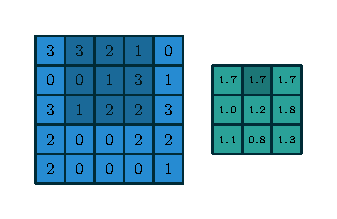
\includegraphics[width=0.32\textwidth]{pdf/numerical_average_pooling_01.pdf}
    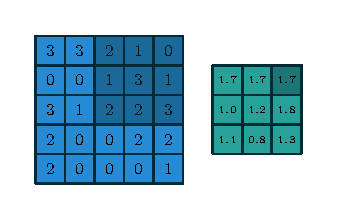
\includegraphics[width=0.32\textwidth]{pdf/numerical_average_pooling_02.pdf}
    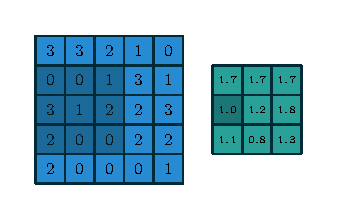
\includegraphics[width=0.32\textwidth]{pdf/numerical_average_pooling_03.pdf}
    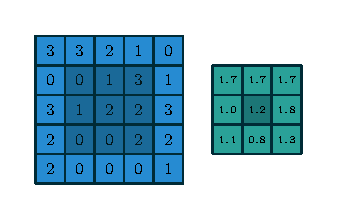
\includegraphics[width=0.32\textwidth]{pdf/numerical_average_pooling_04.pdf}
    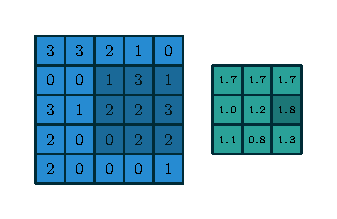
\includegraphics[width=0.32\textwidth]{pdf/numerical_average_pooling_05.pdf}
    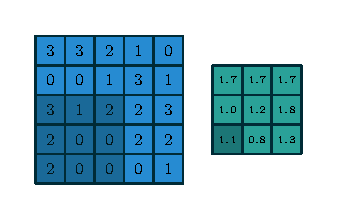
\includegraphics[width=0.32\textwidth]{pdf/numerical_average_pooling_06.pdf}
    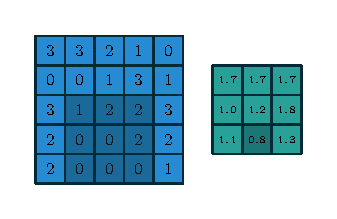
\includegraphics[width=0.32\textwidth]{pdf/numerical_average_pooling_07.pdf}
    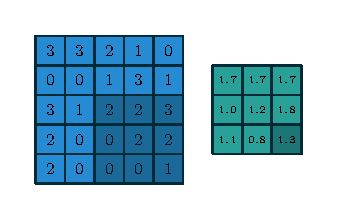
\includegraphics[width=0.32\textwidth]{pdf/numerical_average_pooling_08.pdf}
    \caption{\label{fig:numerical_average_pooling} Computing the output values
        of a $3 \times 3$ average pooling operation on a $5 \times 5$ input
        using $1 \times 1$ strides.}
\end{figure}

\begin{figure}[p]
    \centering
    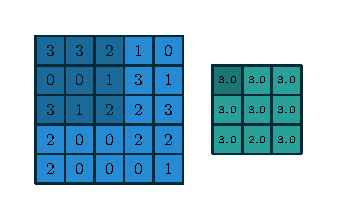
\includegraphics[width=0.32\textwidth]{pdf/numerical_max_pooling_00.pdf}
    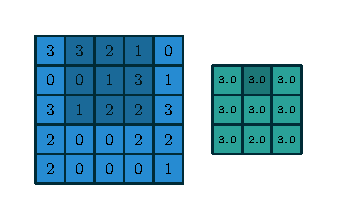
\includegraphics[width=0.32\textwidth]{pdf/numerical_max_pooling_01.pdf}
    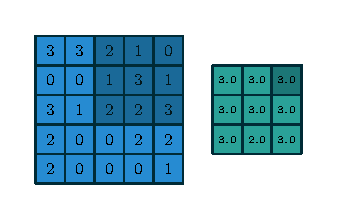
\includegraphics[width=0.32\textwidth]{pdf/numerical_max_pooling_02.pdf}
    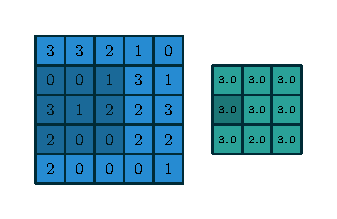
\includegraphics[width=0.32\textwidth]{pdf/numerical_max_pooling_03.pdf}
    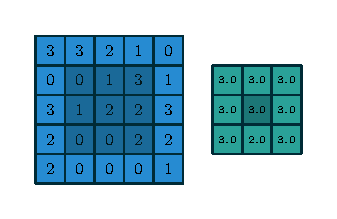
\includegraphics[width=0.32\textwidth]{pdf/numerical_max_pooling_04.pdf}
    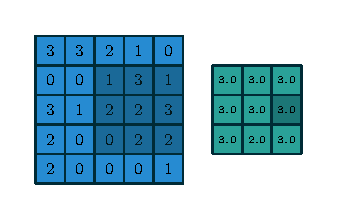
\includegraphics[width=0.32\textwidth]{pdf/numerical_max_pooling_05.pdf}
    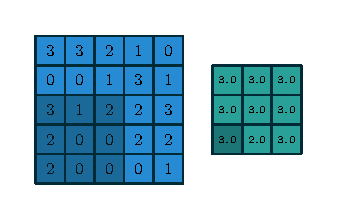
\includegraphics[width=0.32\textwidth]{pdf/numerical_max_pooling_06.pdf}
    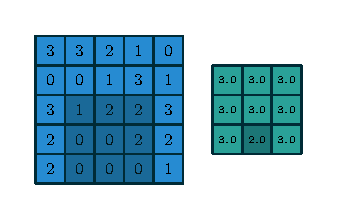
\includegraphics[width=0.32\textwidth]{pdf/numerical_max_pooling_07.pdf}
    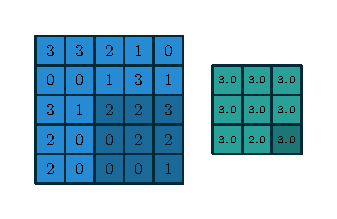
\includegraphics[width=0.32\textwidth]{pdf/numerical_max_pooling_08.pdf}
    \caption{\label{fig:numerical_max_pooling} Computing the output values of a
        $3 \times 3$ max pooling operation on a $5 \times 5$ input using $1
        \times 1$ strides.}
\end{figure}

\subsection{Convolution arithmetic}

The analysis of the relationship between convolutional layer properties is
eased by the fact that they do not interact across axes, i.e., the choice of
kernel size, stride and zero padding along axis $j$ only affects the output
size of axis $j$. Because of that, this chapter focuses on the following
simplified setting to facilitate the analysis and the visualization, but keep
in mind that the results outlined here also generalize to the N-D and
non-square cases:

\begin{itemize}
    \item 2-D discrete convolutions ($N = 2$),
    \item square inputs ($i_1 = i_2 = i$),
    \item square kernel size ($k_1 = k_2 = k$),
    \item same strides along both axes ($s_1 = s_2 = s$),
    \item same zero padding along both axes ($p_1 = p_2 = p$).
\end{itemize}


\subsubsection{No zero padding, unit strides}

The simplest case to analyze is when the kernel just slides across every
position of the input (i.e., $s = 1$ and $p = 0$). \autoref{%
fig:no_padding_no_strides} provides an example for $i = 4$ and $k = 3$.

One way of defining the output size in this case is by the number of possible
placements of the kernel on the input. Let's consider the width axis: the kernel
starts on the leftmost part of the input feature map and slides by steps of one
until it touches the right side of the input. The size of the output will be
equal to the number of steps made, plus one, accounting for the initial position
of the kernel (\autoref{fig:no_padding_no_strides_explained}). The same logic
applies for the height axis. More formally, the following relationship between
the parameters of the convolution, the input shape $i$ and the output shape $o$
can be inferred:

\begin{relationship}\label{rel:no_padding_no_strides}
For any $i$ and $k$, and for $s = 1$ and $p = 0$,
\begin{equation*}
    o = (i - k) + 1.
\end{equation*}
\end{relationship}

\begin{figure}[p]
    \centering
    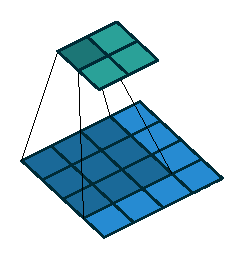
\includegraphics[width=0.24\textwidth]{pdf/no_padding_no_strides_00.pdf}
    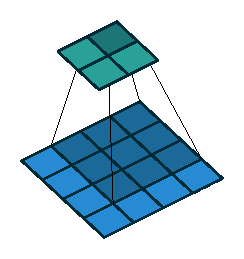
\includegraphics[width=0.24\textwidth]{pdf/no_padding_no_strides_01.pdf}
    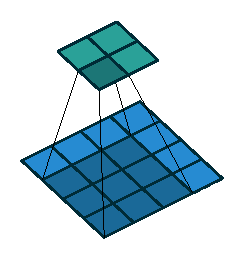
\includegraphics[width=0.24\textwidth]{pdf/no_padding_no_strides_02.pdf}
    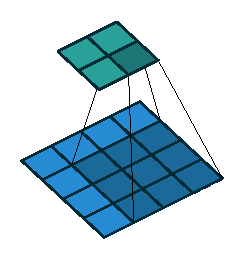
\includegraphics[width=0.24\textwidth]{pdf/no_padding_no_strides_03.pdf}
    \caption{\label{fig:no_padding_no_strides} (No padding, unit strides)
        Convolving a $3 \times 3$ kernel over a $4 \times 4$ input using unit
        strides (i.e., $i = 4$, $k = 3$, $s = 1$ and $p = 0$).}
\end{figure}

\begin{figure}[p]
    \centering
    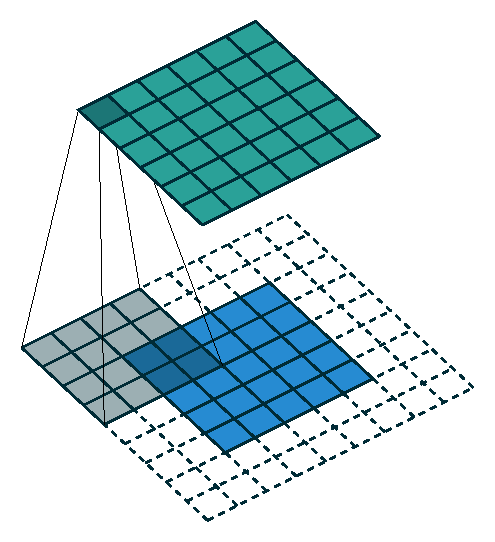
\includegraphics[width=0.24\textwidth]{pdf/arbitrary_padding_no_strides_00.pdf}
    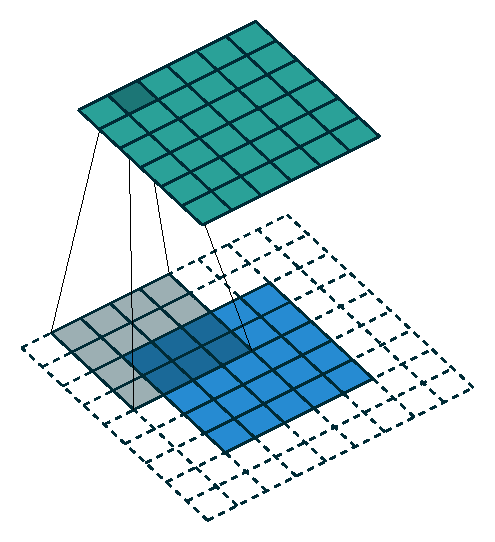
\includegraphics[width=0.24\textwidth]{pdf/arbitrary_padding_no_strides_01.pdf}
    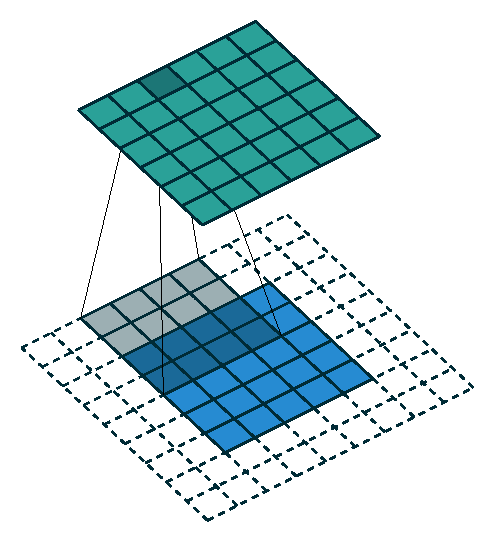
\includegraphics[width=0.24\textwidth]{pdf/arbitrary_padding_no_strides_02.pdf}
    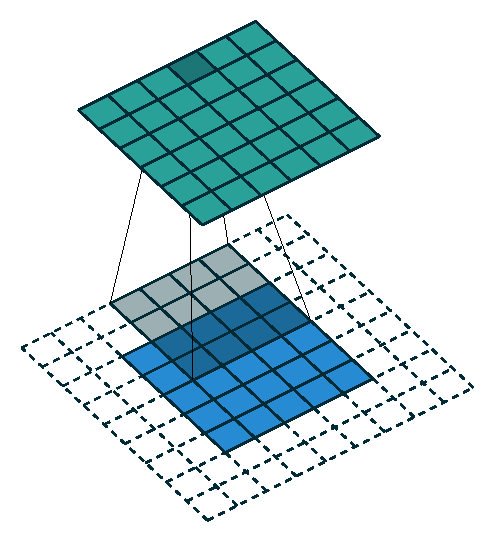
\includegraphics[width=0.24\textwidth]{pdf/arbitrary_padding_no_strides_03.pdf}
    \caption{\label{fig:arbitrary_padding_no_strides} (Arbitrary padding, unit
        strides) Convolving a $4 \times 4$ kernel over a $5 \times 5$ input
        padded with a $2 \times 2$ border of zeros using unit strides (i.e.,
        $i = 5$, $k = 4$, $s = 1$ and $p = 2$).}
\end{figure}

\begin{figure}[p]
    \centering
    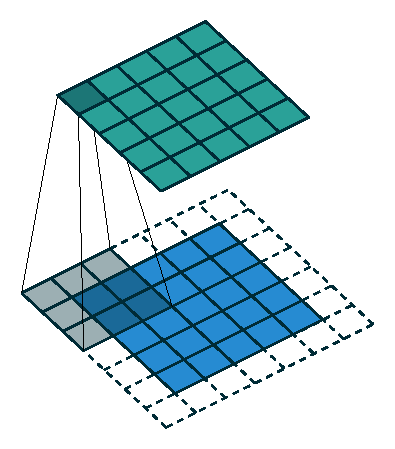
\includegraphics[width=0.24\textwidth]{pdf/same_padding_no_strides_00.pdf}
    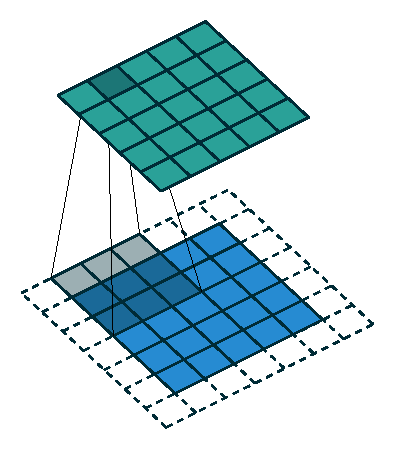
\includegraphics[width=0.24\textwidth]{pdf/same_padding_no_strides_01.pdf}
    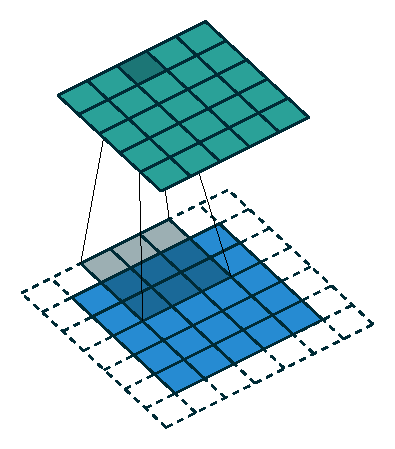
\includegraphics[width=0.24\textwidth]{pdf/same_padding_no_strides_02.pdf}
    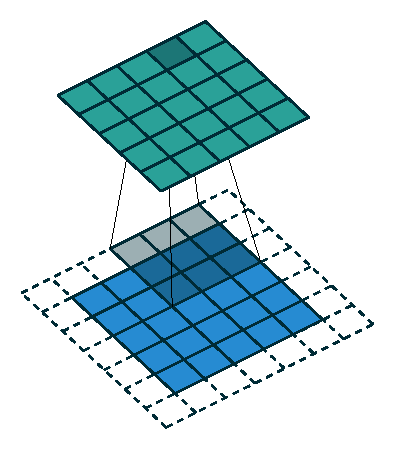
\includegraphics[width=0.24\textwidth]{pdf/same_padding_no_strides_03.pdf}
    \caption{\label{fig:same_padding_no_strides} (Half padding, unit strides)
        Convolving a $3 \times 3$ kernel over a $5 \times 5$ input using half
        padding and unit strides (i.e., $i = 5$, $k = 3$, $s = 1$ and $p = 1$).}
\end{figure}

\begin{figure}[p]
    \centering
    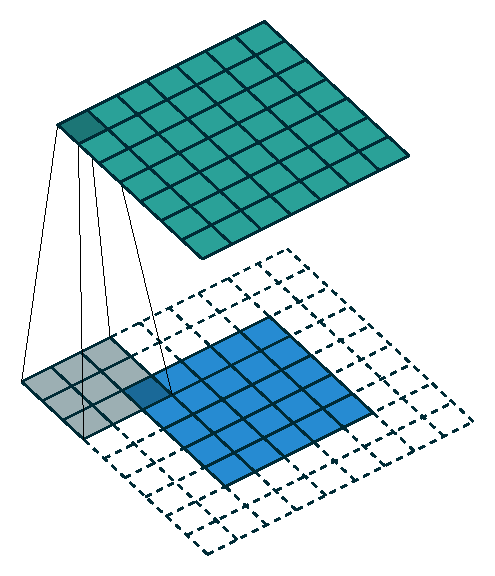
\includegraphics[width=0.24\textwidth]{pdf/full_padding_no_strides_00.pdf}
    \includegraphics[width=0.24\textwidth]{pdf/full_padding_no_strides_01.pdf}
    \includegraphics[width=0.24\textwidth]{pdf/full_padding_no_strides_02.pdf}
    \includegraphics[width=0.24\textwidth]{pdf/full_padding_no_strides_03.pdf}
    \caption{\label{fig:full_padding_no_strides} (Full padding, unit strides)
        Convolving a $3 \times 3$ kernel over a $5 \times 5$ input using full
        padding and unit strides (i.e., $i = 5$, $k = 3$, $s = 1$ and $p = 2$).}
\end{figure}

\subsubsection{Zero padding, unit strides}

To factor in zero padding (i.e., only restricting to $s = 1$), let's consider
its effect on the effective input size: padding with $p$ zeros changes the
effective input size from $i$ to $i + 2p$. In the general case,
\autoref{rel:no_padding_no_strides} can then be used to infer the following
relationship:

\begin{relationship}\label{rel:arbitrary_padding_no_strides}
For any $i$, $k$ and $p$, and for $s = 1$,
\begin{equation*}
    o = (i - k) + 2p + 1,
\end{equation*}
\end{relationship}

\noindent \autoref{fig:arbitrary_padding_no_strides} provides an example for $i
= 5$, $k = 4$ and $p = 2$.

In practice, two specific instances of zero padding are used quite extensively
because of their respective properties. Let's discuss them in more detail.

\subsubsection{Half (same) padding}

Having the output size be the same as the input size (i.e., $o = i$) can be a
desirable property:

\begin{relationship}\label{rel:same_padding_no_strides}
For any $i$ and for $k$ odd ($k = 2n + 1, \quad n \in \mathbb{N}$), $s = 1$ and
$p = \lfloor k / 2 \rfloor = n$,
\begin{equation*}
\begin{split}
    o &= i + 2 \lfloor k / 2 \rfloor - (k - 1) \\
      &= i + 2n - 2n \\
      &= i.
\end{split}
\end{equation*}
\end{relationship}

\noindent This is sometimes referred to as {\em half\/} (or {\em same\/})
padding. \autoref{fig:same_padding_no_strides} provides an example for
$i = 5$, $k = 3$ and (therefore) $p = 1$.

\subsubsection{Full padding}

While convolving a kernel generally {\em decreases\/} the output size with
respect to the input size, sometimes the opposite is required. This can be
achieved with proper zero padding:

\begin{relationship}\label{rel:full_padding_no_strides}
For any $i$ and $k$, and for $p = k - 1$ and $s = 1$,
\begin{equation*}
\begin{split}
    o &= i + 2(k - 1) - (k - 1) \\
      &= i + (k - 1).
\end{split}
\end{equation*}
\end{relationship}

\noindent This is sometimes referred to as {\em full\/} padding, because in this
setting every possible partial or complete superimposition of the kernel on the
input feature map is taken into account. \autoref{fig:full_padding_no_strides}
provides an example for $i = 5$, $k = 3$ and (therefore) $p = 2$.

\subsection{No zero padding, non-unit strides}

All relationships derived so far only apply for unit-strided convolutions.
Incorporating non unitary strides requires another inference leap. To
facilitate the analysis, let's momentarily ignore zero padding (i.e., $s > 1$
and $p = 0$). \autoref{fig:no_padding_strides} provides an example for $i =
5$, $k = 3$ and $s = 2$.

Once again, the output size can be defined in terms of the number of possible
placements of the kernel on the input. Let's consider the width axis: the
kernel starts as usual on the leftmost part of the input, but this time it
slides by steps of size $s$ until it touches the right side of the input. The
size of the output is again equal to the number of steps made, plus one,
accounting for the initial position of the kernel
(\autoref{fig:no_padding_strides_explained}). The same logic applies for the
height axis. From this, the following relationship can be inferred:

\begin{relationship}\label{rel:no_padding_strides}
For any $i$, $k$ and $s$, and for $p = 0$,
\begin{equation*}
    o = \left\lfloor \frac{i - k}{s} \right\rfloor + 1.
\end{equation*}
\end{relationship}

\noindent The floor function accounts for the fact that sometimes the last
possible step does {\em not\/} coincide with the kernel reaching the end of the
input, i.e., some input units are left out (see
\autoref{fig:padding_strides_odd} for an example of such a case).

\subsection{Zero padding, non-unit strides}

The most general case (convolving over a zero padded input using non-unit
strides) can be derived by applying \autoref{rel:no_padding_strides} on an
effective input of size $i + 2p$, in analogy to what was done for
\autoref{rel:arbitrary_padding_no_strides}:

\begin{relationship}\label{rel:padding_strides}
For any $i$, $k$, $p$ and $s$,
\begin{equation*}
    o = \left\lfloor \frac{i + 2p - k}{s} \right\rfloor + 1.
\end{equation*}
\end{relationship}

\noindent As before, the floor function means that in some cases a convolution
will produce the same output size for multiple input sizes. More specifically,
if $i + 2p - k$ is a multiple of $s$, then any input size $j = i + a, \quad a
\in \{0,\ldots,s - 1\}$ will produce the same output size. Note that this
ambiguity applies only for $s > 1$.

\autoref{fig:padding_strides} shows an example with $i = 5$, $k = 3$, $s = 2$
and $p = 1$, while \autoref{fig:padding_strides_odd} provides an example for
$i = 6$, $k = 3$, $s = 2$ and $p = 1$. Interestingly, despite having different
input sizes these convolutions share the same output size. While this does not
affect the analysis for {\em convolutions}, this will complicate the analysis
in the case of {\em transposed convolutions}.

\begin{figure}[p]
    \centering
    \includegraphics[width=0.24\textwidth]{pdf/no_padding_strides_00.pdf}
    \includegraphics[width=0.24\textwidth]{pdf/no_padding_strides_01.pdf}
    \includegraphics[width=0.24\textwidth]{pdf/no_padding_strides_02.pdf}
    \includegraphics[width=0.24\textwidth]{pdf/no_padding_strides_03.pdf}
    \caption{\label{fig:no_padding_strides} (No zero padding, arbitrary
        strides) Convolving a $3 \times 3$ kernel over a $5 \times 5$ input
        using $2 \times 2$ strides (i.e., $i = 5$, $k = 3$, $s = 2$ and
        $p = 0$).}
\end{figure}

\begin{figure}[p]
    \centering
    \includegraphics[width=0.24\textwidth]{pdf/padding_strides_00.pdf}
    \includegraphics[width=0.24\textwidth]{pdf/padding_strides_01.pdf}
    \includegraphics[width=0.24\textwidth]{pdf/padding_strides_02.pdf}
    \includegraphics[width=0.24\textwidth]{pdf/padding_strides_03.pdf}
    \caption{\label{fig:padding_strides} (Arbitrary padding and strides)
        Convolving a $3 \times 3$ kernel over a $5 \times 5$ input padded with
        a $1 \times 1$ border of zeros using $2 \times 2$ strides (i.e.,
        $i = 5$, $k = 3$, $s = 2$ and $p = 1$).}
\end{figure}

\begin{figure}[p]
    \centering
    \includegraphics[width=0.24\textwidth]{pdf/padding_strides_odd_00.pdf}
    \includegraphics[width=0.24\textwidth]{pdf/padding_strides_odd_01.pdf}
    \includegraphics[width=0.24\textwidth]{pdf/padding_strides_odd_02.pdf}
    \includegraphics[width=0.24\textwidth]{pdf/padding_strides_odd_03.pdf}
    \caption{\label{fig:padding_strides_odd} (Arbitrary padding and strides)
        Convolving a $3 \times 3$ kernel over a $6 \times 6$ input padded with
        a $1 \times 1$ border of zeros using $2 \times 2$ strides (i.e.,
        $i = 6$, $k = 3$, $s = 2$ and $p = 1$). In this case, the bottom row
        and right column of the zero padded input are not covered by the
        kernel.}
\end{figure}

\begin{figure}[p]
    \centering
    \begin{subfigure}[t]{0.48\textwidth}
        \centering
        \begin{tikzpicture}[scale=.35,every node/.style={minimum size=1cm},
                            on grid]
            \draw[fill=blue] (0,0) rectangle (5,5);
            \draw[draw=base03, thick] (0,0) grid (5,5);
            \draw[fill=base02, opacity=0.4] (0,2) rectangle (3,5);
            \draw[step=10mm, base03, thick] (0,2) grid (3,5);
            \draw[draw=base03, ->, thick] (2.6,3.5) to  (3.5,3.5);
            \draw[draw=base03, ->, thick] (3.6,3.5) to  (4.5,3.5);
            \draw[draw=base03, ->, thick] (1.5,2.4) to  (1.5,1.5);
            \draw[draw=base03, ->, thick] (1.5,1.4) to  (1.5,0.5);
        \end{tikzpicture}
        \caption{\label{fig:no_padding_no_strides_explained} The kernel has to
            slide two steps to the right to touch the right side of the input
            (and equivalently downwards).  Adding one to account for the
            initial kernel position, the output size is $3 \times 3$.}
    \end{subfigure}
    ~
    \begin{subfigure}[t]{0.48\textwidth}
        \centering
        \begin{tikzpicture}[scale=.35,every node/.style={minimum size=1cm},
                            on grid]
            \draw[fill=blue] (0,0) rectangle (5,5);
            \draw[draw=base03, thick] (0,0) grid (5,5);
            \draw[fill=base02, opacity=0.4] (0,2) rectangle (3,5);
            \draw[step=10mm, base03, thick] (0,2) grid (3,5);
            \draw[draw=base03, ->, thick] (2.5,3.5) to  (4.5,3.5);
            \draw[draw=base03, ->, thick] (1.5,2.5) to  (1.5,0.5);
        \end{tikzpicture}
        \caption{\label{fig:no_padding_strides_explained} The kernel has to
            slide one step of size two to the right to touch the right side of
            the input (and equivalently downwards).  Adding one to account for
            the initial kernel position, the output size is $2 \times 2$.}
    \end{subfigure}
    \caption{Counting kernel positions.}
\end{figure}

\subsection{Pooling arithmetic}

In a neural network, pooling layers provide invariance to small translations of
the input. The most common kind of pooling is \emph{max pooling}, which
consists in splitting the input in (usually non-overlapping) patches and
outputting the maximum value of each patch. Other kinds of pooling exist, e.g.,
mean or average pooling, which all share the same idea of aggregating the input
locally by applying a nonlinearity to the content of some patches \citep{%
boureau-cvpr-10,boureau-icml-10,boureau-iccv-11,ICML2011Saxe_551}.

Notice that the treatment of convolution arithmetic only relies on the
assumption that some function is repeatedly applied onto subsets of the input.
This means that the relationships derived in the previous chapter can be reused
in the case of pooling arithmetic. Since pooling does not involve zero padding,
the relationship describing the general case is as follows:

\begin{relationship}\label{rel:pooling}
For any $i$, $k$ and $s$,
\begin{equation*}
    o = \left\lfloor \frac{i - k}{s} \right\rfloor + 1.
\end{equation*}
\end{relationship}

\noindent This relationship holds for any type of pooling.

\subsection{Transposed convolution arithmetic}\label{sec:transposed_conv}

The need for transposed convolutions generally arises from the desire to use a
transformation going in the opposite direction of a normal convolution, i.e.,
from something that has the shape of the output of some convolution to
something that has the shape of its input while maintaining a connectivity
pattern that is compatible with said convolution. For instance, one might use
such a transformation as the decoding layer of a convolutional autoencoder or to
project feature maps to a higher-dimensional space.

\sloppy
Once again, the convolutional case is considerably more complex than the
fully-connected case, which only requires to use a weight matrix whose shape
has been transposed. However, since every convolution boils down to an
efficient implementation of a matrix operation, the insights gained from the
fully-connected case are useful in solving the convolutional case.

Like for convolution arithmetic, the dissertation about transposed convolution
arithmetic is simplified by the fact that transposed convolution properties
do not interact across axes. The usual simplified setting will be taken in
account, but as before the results outlined generalize to the N-D and
non-square cases.

\subsection{Convolution as a matrix operation}

Take for example the convolution represented in
\autoref{fig:no_padding_no_strides}. If the input and output were to be unrolled
into vectors from left to right, top to bottom, the convolution could be
represented as a sparse matrix $\mathbf{C}$ where the non-zero elements are the
elements $w_{i,j}$ of the kernel (with $i$ and $j$ being the row and column of
the $3x3$ kernel $K=(w_{0,0}..w_{2, 2})$ respectively):
\begin{equation*}
\setcounter{MaxMatrixCols}{20}
\resizebox{.98\hsize}{!}{$%
    \begin{pmatrix}%
    w_{0,0} & w_{0,1} & w_{0,2} & 0       & w_{1,0} & w_{1,1} & w_{1,2} & 0       &
    w_{2,0} & w_{2,1} & w_{2,2} & 0       & 0       & 0       & 0       & 0       \\
    0       & w_{0,0} & w_{0,1} & w_{0,2} & 0       & w_{1,0} & w_{1,1} & w_{1,2} &
    0       & w_{2,0} & w_{2,1} & w_{2,2} & 0       & 0       & 0       & 0       \\
    0       & 0       & 0       & 0       & w_{0,0} & w_{0,1} & w_{0,2} & 0       &
    w_{1,0} & w_{1,1} & w_{1,2} & 0       & w_{2,0} & w_{2,1} & w_{2,2} & 0       \\
    0       & 0       & 0       & 0       & 0       & w_{0,0} & w_{0,1} & w_{0,2} &
    0       & w_{1,0} & w_{1,1} & w_{1,2} & 0       & w_{2,0} & w_{2,1} & w_{2,2} \\
    \end{pmatrix}$}
\end{equation*}

This linear operation takes the input matrix flattened as a 16-dimensional
vector and produces a 4-dimensional vector that is later reshaped as the $2
\times 2$ output matrix.
Using this representation, the backward pass is easily obtained by transposing
$\mathbf{C}$; in other words, the error is backpropagated by multiplying the
loss with $\mathbf{C}^T$. This operation takes a 4-dimensional vector as input
and produces a 16-dimensional vector as output, and its connectivity pattern is
compatible with $\mathbf{C}$ by construction.

Notably, the kernel $\mathbf{w}$ defines both the matrices $\mathbf{C}$ and
$\mathbf{C}^T$ used for the forward and backward passes.

\subsection{Transposed convolution}

Let's now consider what would be required to go the other way around, i.e., map
from a 4-dimensional space to a 16-dimensional space, while keeping the
connectivity pattern of the convolution depicted in
\autoref{fig:no_padding_no_strides}. This operation is known as a {\em
transposed convolution}.

Transposed convolutions -- also called {\em fractionally strided convolutions\/}
-- work by swapping the forward and backward passes of a convolution. One way to
put it is to note that the kernel defines a convolution, but whether it is a
direct convolution or a transposed convolution is determined by how the forward
and backward passes are computed.

For instance, although the kernel $\mathbf{w}$ defines a convolution whose
forward and backward passes are computed by multiplying with $\mathbf{C}$ and
$\mathbf{C}^T$ respectively, it {\em also\/} defines a transposed convolution
whose forward and backward passes are computed by multiplying with
$\mathbf{C}^T$ and $(\mathbf{C}^T)^T = \mathbf{C}$ respectively.\footnote{The
    transposed convolution operation can be thought of as the gradient of {\em
    some\/} convolution with respect to its input, which is usually how
    transposed convolutions are implemented in practice.}

Finally note that it is always possible to emulate a transposed convolution
with a direct convolution. The disadvantage is that it usually involves adding
many columns and rows of zeros to the input, resulting in a much less efficient
implementation.

Building on what has been introduced so far, this section will derive the
properties of each transposed convolution by referring to the direct
convolution with which it shares the kernel, and defining the equivalent direct
convolution.

\subsection{No zero padding, unit strides, transposed}

The simplest way to think about a transposed convolution is by computing the
output shape of the direct convolution for a given input shape first, and then
inverting the input and output shapes for the transposed convolution.

Let's consider the convolution of a $3 \times 3$ kernel on a $4 \times 4$
input with unitary stride and no padding (i.e., $i = 4$, $k = 3$, $s = 1$ and
$p = 0$). As depicted in \autoref{fig:no_padding_no_strides}, this produces a
$2 \times 2$ output. The transpose of this convolution will then have an output
of shape $4 \times 4$ when applied on a $2 \times 2$ input.

Another way to obtain the result of a transposed convolution is to apply an
equivalent -- but much less efficient -- direct convolution. The example
described so far could be tackled by convolving a $3 \times 3$ kernel over a
$2 \times 2$ input padded with a $2 \times 2$ border of zeros using unit
strides (i.e., $i' = 2$, $k' = k$, $s' = 1$ and $p' = 2$), as shown in
\autoref{fig:no_padding_no_strides_transposed}. Notably, the kernel's and
stride's sizes remain the same, but the input of the transposed convolution is
now zero padded.\footnote{Note that although
    equivalent to applying the transposed matrix, this visualization adds a lot
    of zero multiplications in the form of zero padding.  This is done here for
    illustration purposes, but it is inefficient, and software implementations
    will normally not perform the useless zero multiplications.}

One way to understand the logic behind zero padding is to consider the
connectivity pattern of the transposed convolution and use it to guide the
design of the equivalent convolution. For example, the top left pixel of the
input of the direct convolution only contribute to the top left pixel of the
output, the top right pixel is only connected to the top right output pixel,
and so on. To maintain the same connectivity pattern in the equivalent
convolution it is necessary to zero pad the input in such a way that the first
(top-left) application of the kernel only touches the top-left pixel, i.e., the
padding has to be equal to the size of the kernel minus one.

Proceeding in the same fashion it is possible to determine similar observations
for the other elements of the image, giving rise to the following relationship:

\begin{relationship}\label{rel:no_padding_no_strides_transposed}
A convolution described by $s = 1$, $p = 0$ and $k$ has an associated
transposed convolution described by $k' = k$, $s' = s$ and $p' = k - 1$ and its
output size is
\begin{equation*}
    o' = i' + (k - 1).
\end{equation*}
\end{relationship}

Interestingly, this corresponds to a fully padded convolution with unit
strides.

\subsection{Zero padding, unit strides, transposed}

Knowing that the transpose of a non-padded convolution is equivalent to
convolving a zero padded input, it would be reasonable to suppose that the
transpose of a zero padded convolution is equivalent to convolving an input
padded with {\em less\/} zeros. It is indeed the case, as shown in
\autoref{fig:arbitrary_padding_no_strides_transposed} for $i = 5$, $k = 4$ and
$p = 2$.

Formally, the following relationship applies for zero padded convolutions:

\begin{relationship}\label{rel:arbitrary_padding_no_strides_transposed}
A convolution described by $s = 1$, $k$ and $p$ has an
associated transposed convolution described by $k' = k$, $s' = s$ and $p' = k -
p - 1$ and its output size is
\begin{equation*}
    o' = i' + (k - 1) - 2p.
\end{equation*}
\end{relationship}

\begin{figure}[p]
    \centering
    \includegraphics[width=0.24\textwidth]{pdf/no_padding_no_strides_transposed_00.pdf}
    \includegraphics[width=0.24\textwidth]{pdf/no_padding_no_strides_transposed_01.pdf}
    \includegraphics[width=0.24\textwidth]{pdf/no_padding_no_strides_transposed_02.pdf}
    \includegraphics[width=0.24\textwidth]{pdf/no_padding_no_strides_transposed_03.pdf}
    \caption{\label{fig:no_padding_no_strides_transposed} The transpose of
        convolving a $3 \times 3$ kernel over a $4 \times 4$ input using unit
        strides (i.e., $i = 4$, $k = 3$, $s = 1$ and $p = 0$). It is equivalent
        to convolving a $3 \times 3$ kernel over a $2 \times 2$ input padded
        with a $2 \times 2$ border of zeros using unit strides (i.e., $i' = 2$,
        $k' = k$, $s' = 1$ and $p' = 2$).}
\end{figure}

\begin{figure}[p]
    \centering
    \includegraphics[width=0.24\textwidth]{pdf/arbitrary_padding_no_strides_transposed_00.pdf}
    \includegraphics[width=0.24\textwidth]{pdf/arbitrary_padding_no_strides_transposed_01.pdf}
    \includegraphics[width=0.24\textwidth]{pdf/arbitrary_padding_no_strides_transposed_02.pdf}
    \includegraphics[width=0.24\textwidth]{pdf/arbitrary_padding_no_strides_transposed_03.pdf}
    \caption{\label{fig:arbitrary_padding_no_strides_transposed} The transpose
        of convolving a $4 \times 4$ kernel over a $5 \times 5$ input padded
        with a $2 \times 2$ border of zeros using unit strides (i.e., $i = 5$,
        $k = 4$, $s = 1$ and $p = 2$). It is equivalent to convolving a $4
        \times 4$ kernel over a $6 \times 6$ input padded with a $1 \times 1$
        border of zeros using unit strides (i.e., $i' = 6$, $k' = k$, $s' = 1$
        and $p' = 1$).}
\end{figure}

\begin{figure}[p]
    \centering
    \includegraphics[width=0.24\textwidth]{pdf/same_padding_no_strides_transposed_00.pdf}
    \includegraphics[width=0.24\textwidth]{pdf/same_padding_no_strides_transposed_01.pdf}
    \includegraphics[width=0.24\textwidth]{pdf/same_padding_no_strides_transposed_02.pdf}
    \includegraphics[width=0.24\textwidth]{pdf/same_padding_no_strides_transposed_03.pdf}
    \caption{\label{fig:same_padding_no_strides_transposed} The transpose of
        convolving a $3 \times 3$ kernel over a $5 \times 5$ input using half
        padding and unit strides (i.e., $i = 5$, $k = 3$, $s = 1$ and $p = 1$).
        It is equivalent to convolving a $3 \times 3$ kernel over a $5 \times 5$
        input using half padding and unit strides (i.e., $i' = 5$, $k' = k$, $s'
        = 1$ and $p' = 1$).}
\end{figure}

\subsubsection{Half (same) padding, transposed}

By applying the same inductive reasoning as before, it is reasonable to expect
that the equivalent convolution of the transpose of a half padded convolution
is itself a half padded convolution, given that the output size of a half
padded convolution is the same as its input size. Thus the following relation
applies:

\begin{relationship}\label{rel:half_padding_no_strides_transposed}
A convolution described by $k = 2n + 1, \quad n \in \mathbb{N}$, $s = 1$ and $p
= \lfloor k / 2 \rfloor = n$ has an associated transposed convolution described
by $k' = k$, $s' = s$ and $p' = p$ and its output size is
\begin{equation*}
\begin{split}
    o' &= i' + (k - 1) - 2p \\
       &= i' + 2n - 2n \\
       &= i'.
\end{split}
\end{equation*}
\end{relationship}

\noindent\autoref{fig:same_padding_no_strides_transposed} provides an example
for $i = 5$, $k = 3$ and (therefore) $p = 1$.

\subsubsection{Full padding, transposed}

Knowing that the equivalent convolution of the transpose of a non-padded
convolution involves full padding, it is unsurprising that the equivalent of
the transpose of a fully padded convolution is a non-padded convolution:

\begin{relationship}\label{rel:full_padding_no_strides_transposed}
A convolution described by $s = 1$, $k$ and $p = k - 1$ has an
associated transposed convolution described by $k' = k$, $s' = s$ and $p' = 0$
and its output size is
\begin{equation*}
\begin{split}
    o' &= i' + (k - 1) - 2p \\
       &= i' - (k - 1).
\end{split}
\end{equation*}
\end{relationship}

\noindent\autoref{fig:full_padding_no_strides_transposed} provides an example
for $i = 5$, $k = 3$ and (therefore) $p = 2$.

\begin{figure}[p]
    \centering
    \includegraphics[width=0.24\textwidth]{pdf/full_padding_no_strides_transposed_00.pdf}
    \includegraphics[width=0.24\textwidth]{pdf/full_padding_no_strides_transposed_01.pdf}
    \includegraphics[width=0.24\textwidth]{pdf/full_padding_no_strides_transposed_02.pdf}
    \includegraphics[width=0.24\textwidth]{pdf/full_padding_no_strides_transposed_03.pdf}
    \caption{\label{fig:full_padding_no_strides_transposed} The transpose of
        convolving a $3 \times 3$ kernel over a $5 \times 5$ input using full
        padding and unit strides (i.e., $i = 5$, $k = 3$, $s = 1$ and $p = 2$).
        It is equivalent to convolving a $3 \times 3$ kernel over a $7 \times
        7$ input using unit strides (i.e., $i' = 7$, $k' = k$, $s' = 1$ and
        $p' = 0$).}
\end{figure}

\begin{figure}[p]
    \centering
    \includegraphics[width=0.24\textwidth]{pdf/no_padding_strides_transposed_00.pdf}
    \includegraphics[width=0.24\textwidth]{pdf/no_padding_strides_transposed_01.pdf}
    \includegraphics[width=0.24\textwidth]{pdf/no_padding_strides_transposed_02.pdf}
    \includegraphics[width=0.24\textwidth]{pdf/no_padding_strides_transposed_03.pdf}
    \caption{\label{fig:no_padding_strides_transposed} The transpose of
        convolving a $3 \times 3$ kernel over a $5 \times 5$ input using $2
        \times 2$ strides (i.e., $i = 5$, $k = 3$, $s = 2$ and $p = 0$). It is
        equivalent to convolving a $3 \times 3$ kernel over a $2 \times 2$ input
        (with $1$ zero inserted between inputs) padded with a $2 \times 2$
        border of zeros using unit strides (i.e., $i' = 2$, $\tilde{i}' = 3$,
        $k' = k$, $s' = 1$ and $p' = 2$).}
\end{figure}

\begin{figure}[p]
    \centering
    \includegraphics[width=0.24\textwidth]{pdf/padding_strides_transposed_00.pdf}
    \includegraphics[width=0.24\textwidth]{pdf/padding_strides_transposed_01.pdf}
    \includegraphics[width=0.24\textwidth]{pdf/padding_strides_transposed_02.pdf}
    \includegraphics[width=0.24\textwidth]{pdf/padding_strides_transposed_03.pdf}
    \caption{\label{fig:padding_strides_transposed} The transpose of convolving
        a $3 \times 3$ kernel over a $5 \times 5$ input padded with a $1 \times
        1$ border of zeros using $2 \times 2$ strides (i.e., $i = 5$, $k = 3$,
        $s = 2$ and $p = 1$). It is equivalent to convolving a $3 \times 3$
        kernel over a $2 \times 2$ input (with $1$ zero inserted between
        inputs) padded with a $1 \times 1$ border of zeros using unit strides
        (i.e., $i' = 3$, $\tilde{i}' = 5$, $k' = k$, $s' = 1$ and $p' = 1$).}
\end{figure}

\begin{figure}[t]
    \centering
    \includegraphics[width=0.24\textwidth]{pdf/padding_strides_odd_transposed_00.pdf}
    \includegraphics[width=0.24\textwidth]{pdf/padding_strides_odd_transposed_01.pdf}
    \includegraphics[width=0.24\textwidth]{pdf/padding_strides_odd_transposed_02.pdf}
    \includegraphics[width=0.24\textwidth]{pdf/padding_strides_odd_transposed_03.pdf}
    \caption{\label{fig:padding_strides_odd_transposed} The transpose of
        convolving a $3 \times 3$ kernel over a $6 \times 6$ input padded with
        a $1 \times 1$ border of zeros using $2 \times 2$ strides (i.e., $i =
        6$, $k = 3$, $s = 2$ and $p = 1$). It is equivalent to convolving a $3
        \times 3$ kernel over a $2 \times 2$ input (with $1$ zero inserted
        between inputs) padded with a $1 \times 1$ border of zeros (with an
        additional border of size $1$ added to the top and right edges) using
        unit strides (i.e., $i' = 3$, $\tilde{i}' = 5$, $a = 1$, $k' = k$,
        $s' = 1$ and $p' = 1$).}
\end{figure}


\subsection{No zero padding, non-unit strides, transposed}

Using the same kind of inductive logic as for zero padded convolutions, one
might expect that the transpose of a convolution with $s > 1$ involves an
equivalent convolution with $s < 1$. As will be explained, this is a valid
intuition, which is why transposed convolutions are sometimes called {\em
fractionally strided convolutions}.
\autoref{fig:no_padding_strides_transposed} provides an example for $i = 5$, $k
= 3$ and $s = 2$ which helps understand what fractional strides involve: zeros
are inserted {\em between\/} input units, which makes the kernel move around at
a slower pace than with unit strides.\footnote{Doing so is inefficient and
    real-world implementations avoid useless multiplications by zero, but
    conceptually it is how the transpose of a strided convolution can be
    thought of.}

For the moment, it will be assumed that the convolution is non-padded ($p = 0$)
and that its input size $i$ is such that $i - k$ is a multiple of $s$. In that
case, the following relationship holds:

\begin{relationship}\label{rel:no_padding_strides_transposed}
A convolution described by $p = 0$, $k$ and $s$ and whose input
size is such that $i - k$ is a multiple of $s$, has an associated transposed
convolution described by $\tilde{i}'$, $k' = k$, $s' = 1$ and $p' = k - 1$,
where $\tilde{i}'$ is the size of the stretched input obtained by adding
$s - 1$ zeros between each input unit, and its output size is
\begin{equation*}
\begin{split}
    o' = s (i' - 1) + k.
\end{split}
\end{equation*}
\end{relationship}

\subsection{Zero padding, non-unit strides, transposed}

When the convolution's input size $i$ is such that $i + 2p - k$ is a multiple
of $s$, the analysis can be extended to the zero padded case by combining
\autoref{rel:arbitrary_padding_no_strides_transposed} and
\autoref{rel:no_padding_strides_transposed}:

\begin{relationship}\label{rel:padding_strides_transposed}
    A convolution described by $k$, $s$ and $p$ and whose
    input size $i$ is such that $i + 2p - k$ is a multiple of $s$ has an
    associated transposed convolution described by $\tilde{i}'$, $k' = k$, $s'
    = 1$ and $p' = k - p - 1$, where $\tilde{i}'$ is the size of the stretched
    input obtained by adding $s - 1$ zeros between each input unit, and its
    output size is
    \begin{equation*}
    \begin{split}
        o' = s (i' - 1) + k - 2p.
    \end{split}
    \end{equation*}
\end{relationship}

\noindent\autoref{fig:padding_strides_transposed} provides an example for $i =
5$, $k = 3$, $s = 2$ and $p = 1$.

The constraint on the size of the input $i$ can be relaxed by introducing
another parameter $a \in \{0, \ldots, s - 1\}$ that allows to distinguish
between the $s$ different cases that all lead to the same $i'$:

\begin{relationship}\label{rel:padding_strides_transposed_odd}
    A convolution described by $k$, $s$ and $p$ has an
    associated transposed convolution described by $a$, $\tilde{i}'$, $k' = k$,
    $s' = 1$ and $p' = k - p - 1$, where $\tilde{i}'$ is the size of the
    stretched input obtained by adding $s - 1$ zeros between each input unit,
    and $a = (i + 2p - k) \mod s$ represents the number of zeros added to the
    top and right edges of the input, and its output size is
    \begin{equation*}
    \begin{split}
        o' = s (i' - 1) + a + k - 2p.
    \end{split}
    \end{equation*}
\end{relationship}

\noindent\autoref{fig:padding_strides_odd_transposed} provides an example for
$i = 6$, $k = 3$, $s = 2$ and $p = 1$.

%================================== SECTION ==================================
\section{Recurrent networks}\label{sec:rnn}
% A biological neuron takes around $10^{-3}$ seconds to perform one operation,
% and the number of neurons
% whereas a modern GPU can process up to NN DATA per second~\citep{NVIDIA}.
% Nonetheless, many tasks that are trivial for humans prove to be extremely
% complicated for computers. Why is that? The power of the brain lies in its
% large number of connections.\cite{SOMETHING}
%
It is well known that the brain is organized in functional areas and sub-areas
that process the incoming signal in an incremental fashion. These areas of the
brain are typically connected both in a \emph{feedforward}, i.e., towards
neurons belonging to deeper (i.e., further away from the sensory input) layers,
and in a \emph{feedback} fashion (i.e., to previous layers in the hierarchy).
This is believed to help processing temporal data and allow for an iterative
refinement of the computation.

Similarly, ANNs are not constrained to process the input data in a feedforward
way. Recurrent Neural Networks (RNNs) implement feedback loops
(see~\autoref{fig:RNN_loop} \footnote{This and the following RNN figures, are
    taken or modified from the awesome introduction to RNNs and LSTMs by Chris
    Olah~\citep{olah2015rnns}}) that propagate some information from one step to
the next. It is customary to refer to these steps as time-steps, as RNNs are
often considered in the context of a discretized time evolving domain, but
nothing prevents from using RNNs with any kind of sequential data.

\begin{figure}[t]
    \centering
    \includegraphics[width=0.15\textwidth]{pdf/RNN_loop.pdf}
    \caption{A Recurrent Neural Network (RNN).\label{fig:RNN_loop}}
\end{figure}

\begin{figure}[t!]
    \centering
    \includegraphics[width=0.7\textwidth]{pdf/RNN_unrolled.pdf}
    \caption{A Recurrent Neural Network unrolled for $t$%
             steps.\label{fig:RNN_unrolled}}
\end{figure}

Suppose to model some sequential data $x_0, x_1, \dots , x_t, x_{t+1}, \dots$
such as an English sentence. At time $t$ it is possible to model the
probability distribution over a dictionary of English words, conditioned on the
words seen up that moment -- namely $x_0, x_1, \dots , x_{t-1}$. This can be
used, for instance, in a smart keyboard application to suggest the next most
probable words to the user or, in an automatic help desk, to generate a
meaningful answer to a question.

It might not be immediately obvious what it means in practice to put a loop in
an ANN and how to backpropagate through it. To better comprehend how RNNs work
it is useful to consider its behavior explicitly by \emph{unrolling} the RNN,
as shown in~\autoref{fig:RNN_unrolled}

\noindent An RNN applies the same model to each time step of the sequence or,
equivalently, applies different models at each time step, which share their
weights. This is similar to what CNNs do over space with convolutions, but is
rather done over time with feedback connections.

The activation of an RNN (see~\autoref{fig:RNN_unrolled}) at time $t$ depends
on the input at time $t$ as well as on the information coming from the previous
step $t-1$. RNNs have a very simple internal structure, that usually amounts to
applying some affine transformation to the input and to the previous output,
and computing some non-linearity (typically a tanh) of their sum.

\begin{figure}[t]
    \centering
    \includegraphics[width=0.7\textwidth]{pdf/RNN_internals.pdf}
    \includegraphics[width=0.7\textwidth]{pdf/LSTM_notation.pdf}
    \caption{The internal structure of an RNN.\label{fig:RNN_internals}}
\end{figure}

To train it it suffices to unroll the computation graph and use the
backpropagation algorithm (see~\autoref{sec:backprop}) to proceed from the most
recent time step, backward in time. This algorithm is usually referred to as
\emph{Backpropagation through time (BPTT)}.

The problem of BPTT is that it requires the application of the chain rule all
the way from the current time step to $t = 0$ to propagate the gradients
through time.  This results in a long chain of products that can easily go to
infinity or become zero if the elements of the multiplication are greater or
smaller than $1$ respectively. These two issues, i.e., going to infinity and
becoming zero, are known in the literature as \emph{exploding gradient} and
\emph{vanishing gradient} respectively, and have been studied extensively in
the past~\citep[see e.g., ][]{Hochreiter91,Bengio-trnn93}. The first one can be
partially addressed by \emph{clipping the gradient} when it becomes too large,
but the second is not easy to overcome and can make training these kind of
models very hard if not impossible.

\subsection{Long Short Term Memory}
\begin{figure}[t]
    \centering
    \includegraphics[width=0.7\textwidth]{pdf/LSTM.pdf}
    \caption{A Long Short Term Memory (LSTM).\label{fig:LSTM}}
\end{figure}

Long Short Term Memory (LSTM) networks (see~\autoref{fig:LSTM}) have been
proposed to solve (or at least alleviate) the problems of RNNs in modeling
long term dependencies. LSTMs have been designed to have an internal memory,
or~\emph{state}, that can be updated and consulted at each time step. As
opposed to vanilla RNNs, this allows LSTMs to separate their output from the
information they want to carry over to future steps.

\begin{figure}[t]
    \centering
    \includegraphics[width=0.5\textwidth]{pdf/LSTM_state.pdf}
    \caption{The internal state of LSTMs.\label{fig:LSTM_state}}
\end{figure}

\autoref{fig:LSTM_state} highlights the internal memory path. It can be seen
how the internal memory of the previous time step $C_{t-1}$ is carried over to
the current time step, where it is updated through a multiplicative and an
additive interaction and concurs to determine the current state of the memory
$C_t$. This is then, once again, propagated to the next time step.
% The internal memory is updated at each time step
% with the rest of the architecture.

\begin{figure}[p]
    \centering
    \includegraphics[width=0.5\textwidth]{pdf/LSTM_forget_gate.pdf}
    \caption{The LSTM forget gate.\label{fig:LSTM_forget_gate}}
\end{figure}
\begin{figure}[p]
    \centering
    \includegraphics[width=0.5\textwidth]{pdf/LSTM_input_gate.pdf}
    \caption{The LSTM input gate.\label{fig:LSTM_input_gate}}
\end{figure}
\begin{figure}[p]
    \centering
    \includegraphics[width=0.5\textwidth]{pdf/LSTM_output_gate.pdf}
    \caption{The LSTM output gate.\label{fig:LSTM_output_gate}}
\end{figure}

LSTMs interact with memory through \emph{gates}, computational nodes that
determine the behavior of the model. The \emph{forget~gate}~(\autoref{%
fig:LSTM_forget_gate}) determines how much of the previous step's memory to
forget or, equivalently, how much of the previous state to retain.  This is
modeled through a sigmoid layer (depicted as $\sigma$) that takes the current
input $x_t$ and the output of the previous step $h_{t-1}$ and produces an
activation vector between $0$ and $1$

\begin{equation}\label{eq:LSTM_forget_gate}
    f_t = \sigma\left(W_f \cdot \left[h_{t-1}, x_t\right] + b_f \right),
\end{equation}

\noindent this activation is multiplied by the previous state $C_{t-1}$ and
results in an intermediate memory state where some of the activations can be
weaker than those in $C_{t-1}$ and some others are potentially zeroed out.

The forget gate allows the LSTM to discard information that is not relevant
anymore. Symmetrically, LSTMs have a mechanism to add new information to the
memory. This behavior is controlled by an \emph{input~gate}~(\autoref{%
fig:LSTM_input_gate}) that modulates the amount of the current input that is
going to be stored in the memory. This operation is split over two computation
paths: similarly to the forget gate, the input gate takes the current input
$x_t$ and the output of the previous step $h_{t-1}$ and exploits a sigmoid
layer to produce an activation vector between $0$ and $1$. Simultaneously, a
tanh layer generates a state update $\tilde C_t$ between $-1$ and $1$. This is
governed by the equations

\begin{equation}\label{eq:LSTM_input_gate}
\begin{split}
    i_t &= \sigma\left(W_i \cdot \left[h_{t-1}, x_t\right] + b_i \right)\\
    \tilde C_t &= tanh \left(W_c \cdot \left[h_{t-1}, x_t\right] + b_c \right).
\end{split}
\end{equation}

The input gate modulates how much of this state update will be applied to the
old state to generate the current state. The forget gate $f_t$ and the input
gate $i_t$, together with the state update $\tilde C_t$ and the previous state
$C_{t-1}$ fully determine the state at time $t$ through

\begin{equation}\label{eq:LSTM_state_update}
    C_t = f_t \hadamard C_{t-1} + i_t \hadamard \tilde C_t.
\end{equation}

The last gate of LSTMs is the \emph{output~gate}~(\autoref{%
fig:LSTM_output_gate}) $o_t$ that, as the name reveals, manipulates the output
of the LSTM at time $t$. The usual sigmoid layer determines the state of the
output gate

\begin{equation}\label{eq:LSTM_output_gate}
\begin{split}
    o_t &= \sigma\left(W_o \cdot \left[h_{t-1}, x_t\right] + b_o \right)\\
    h_t &= o_t \hadamard tanh \left(C_t\right),
\end{split}
\end{equation}

\noindent and the memory resulting from the transformations due to the forget and
input gates goes through a tanh nonlinearity and is multiplied by the output
gate to finally produce the output.

Putting it all together, the equations that govern the behavior of an LSTM are

\begin{equation}\label{eq:LSTM}
\begin{split}
    i_t &= \sigma\left(W_i \cdot \left[h_{t-1}, x_t\right] + b_i \right)\\
    f_t &= \sigma\left(W_f \cdot \left[h_{t-1}, x_t\right] + b_f \right)\\
    \tilde C_t &= tanh \left(W_c \cdot \left[h_{t-1}, x_t\right] + b_c \right)\\
    C_t &= f_t \hadamard C_{t-1} + i_t \hadamard \tilde C_t\\
    o_t &= \sigma\left(W_o \cdot \left[h_{t-1}, x_t\right] + b_o \right)\\
    h_t &= o_t \hadamard tanh \left(C_t\right).
\end{split}
\end{equation}


\subsubsection{LSTMs with peepholes}

\cite{gers2000recurrent} suggests one variant of LSTMs where the gates also
have information about the state of the LSTM. Note that, as illustrated
in~\autoref{fig:LSTM_peepholes}, the output gate peeps into $C_t$, i.e., the
state after the input and forget gate updates

\begin{figure}[t]
    \centering
    \includegraphics[width=0.5\textwidth]{pdf/LSTM_peepholes.pdf}
    \caption{LSTM with peepholes.\label{fig:LSTM_peepholes}}
\end{figure}

\begin{equation}\label{eq:LSTM_peepholes}
\begin{split}
    i_t &= \sigma\left(W_i \cdot \left[h_{t-1}, x_t\right] +
        W_{ic} \circ C_{t-1} + b_i \right)\\
    f_t &= \sigma\left(W_f \cdot \left[h_{t-1}, x_t\right] +
        W_{fc} \circ C_{t-1} + b_f \right)\\
    \tilde C_t &= tanh \left(W_c \cdot \left[h_{t-1}, x_t\right] +
        b_c \right)\\
    C_t &= f_t \hadamard C_{t-1} + i_t \hadamard \tilde C_t\\
    o_t &= \sigma\left(W_o \cdot \left[h_{t-1}, x_t\right] +
        W_{oc} \hadamard C_{t-1} + b_o \right)\\
    h_t &= o_t \hadamard tanh \left(C_t\right).
\end{split}
\end{equation}


\subsubsection{LSTMs with coupled forget and input gates}\label{sec:LSTM_coupled}

Another variant of LSTMs~\citep{Greff-et-al-arxiv2015} replaces the input gate
with $1 - f_t$ (see~\autoref{fig:LSTM_coupled}), so that the forget gate governs
both behaviors. This boils down to forgetting only when a new
input is going to be written. The modified state update equation is

\begin{equation}\label{eq:LSTM_coupled}
    C_t = f_t \hadamard C_{t-1} + (1 - f_t) \hadamard \tilde C_t.
\end{equation}

\begin{figure}[t]
    \centering
    \includegraphics[width=0.5\textwidth]{pdf/LSTM_coupled.pdf}
    \caption{LSTM with coupled forget and input gate.\label{fig:LSTM_coupled}}
\end{figure}


\subsection{Gated Recurrent Unit (GRU)}

In 2014 \cite{Cho2014a} proposed a new kind of recurrent network called Gated
Recurrent Unit (GRU) (see~\autoref{fig:GRU}) with less gates than LSTMs and a
different internal structure. Along the lines of \autoref{sec:LSTM_coupled}, in
GRUs the forget and input gates are coupled into an~\emph{update gate} $z_t$.
The memory and output are also merged into a single state and the internal
structure is modified to cope with these changes

\begin{equation}\label{eq:GRU}
\begin{split}
    z_t &= \sigma \left( W_z \cdot \left[h_{t-1}, x_t\right]\right) \\
    r_t &= \sigma \left( W_r \cdot \left[h_{t-1}, x_t\right]\right) \\
    \tilde h_t &= tanh \left(W_o \cdot \left[r_t \hadamard h_{t-1}, x_t\right]
        \right) \\
    h_t &= (1-z_t) \hadamard h_{t-1} + (z_t) \hadamard \tilde h_t.
\end{split}
\end{equation}

The advantage of GRUs over LSTMs is the smaller number of gates that makes them
less memory as well as computationally intense, which is often a critical
aspect for ANNs. GRUs have been shown to perform as well as LSTMs in some
settings (see~\cite{Chung-et-al-NIPSDL2014-small}).

\begin{figure}[pt]
    \centering
    \includegraphics[width=0.5\textwidth]{pdf/GRU.pdf}
    \caption{Gated Recurrent Units (GRUs).\label{fig:GRU}}
\end{figure}
